\documentclass[aspectratio=169]{beamer}
\usepackage{german}
\usepackage[utf8]{inputenc} %for windows
\usepackage[T1]{fontenc}
\usepackage{textcomp}
\usepackage{gensymb}
\usepackage{graphicx}
\usepackage{tikz}
\usepackage{pgfplots}
\usepackage{xcolor}
\usepackage{siunitx}
\usepackage{listings}
\usepackage{caption, subcaption}
\usepackage{verbatim}
\usepackage{eso-pic} %to draw on top right corner

%define hsr colors
\definecolor{hsrBlue}{RGB}{000,101,163}
\definecolor{hsrHematite}{RGB}{110,028,080}
\definecolor{hsrLakeGreen}{RGB}{084,140,134}
\definecolor{hsrReed}{RGB}{123,105,081}
\definecolor{hsrPetrol}{RGB}{000,115,141}
\definecolor{hsrBasswood}{RGB}{186,189,093}
\definecolor{hsrGray}{RGB}{198,199,200}
\definecolor{hsrBlack}{RGB}{026,023,027}

%design & color
\usetheme[width=2.2cm]{PaloAlto}
\usecolortheme{beaver}
\useinnertheme{circles}
\usefonttheme[onlymath]{serif}
\setbeamercolor{section in sidebar}{fg=hsrBlack}
\setbeamercolor{itemize item}{fg=hsrBlue}
\setbeamercolor{itemize subitem}{fg=hsrLakeGreen}
\setbeamercolor{item projected}{fg=white,bg=hsrBlack}
\setbeamercolor{title in sidebar}{fg=hsrBlack}
\setbeamercolor{author in sidebar}{fg=hsrBlue} 
\setbeamercolor{caption name}{fg=hsrBlue}
\setbeamercolor*{title}{fg=hsrBlue}
\setbeamercolor{frametitle}{fg=hsrBlue, bg=hsrGray!15!white}
\setbeamercolor{sidebar}{bg=hsrGray!15!white}
\setbeamercolor{logo}{bg=hsrGray!0!white}

%disable navigation symbols
\beamertemplatenavigationsymbolsempty
%slide numbers
\setbeamertemplate{footline}[frame number]

%used for drawing n(r)-Area
\definecolor{lGray}{gray}{0.8}
\definecolor{llGray}{gray}{0.9}
\usepgfplotslibrary{fillbetween}
\usetikzlibrary{fadings}

\definecolor{listinggray}{gray}{0.9}
\definecolor{lbcolor}{rgb}{0.97,0.97,0.97}
\definecolor{lightGray}{gray}{0.1}

\definecolor{cOrange}{HTML}{996633}
\definecolor{clOrange}{HTML}{DBB48D}
\definecolor{cBlue}{HTML}{336699}
\definecolor{clBlue}{HTML}{A0BCD8}
\definecolor{cGreen}{HTML}{339966}
\definecolor{clGreen}{HTML}{94D4B4}
\definecolor{cRed}{HTML}{993333}
\definecolor{clRed}{HTML}{D0B0B0}
\definecolor{cGray}{gray}{0.4}
\definecolor{clGray}{gray}{0.96}

\tikzset{>=stealth}

\newcommand{\eurobot}{$\text{Eurobot}^\text{open}$\ }

% ----- lstListings (C++ code with syntax highlighting) -----
\lstset{
	backgroundcolor=\color{lbcolor},
	xleftmargin=0.5cm,
	xrightmargin=0.5cm,
	tabsize=2,
	language=C++,
	captionpos=b,
	frame=none,
	numbers=none,
	numberstyle=\tiny,
	numbersep=5pt,
	breaklines=true,
	breakautoindent=true, 
	breakindent=20pt,
	breakatwhitespace=true,
	showstringspaces=false,
	%prebreak=\raisebox{0ex}[0ex][0ex]{\ensuremath{\color{cRed}\rhookswarrow}},
	postbreak=\raisebox{0ex}[0ex][0ex]{\ensuremath{\color{cRed}\lhookrightarrow\space}},
	basicstyle=\ttfamily,
	identifierstyle=\color{black},
	keywordstyle=\color{cRed},
	commentstyle=\color{cGreen},
	stringstyle=\color{cOrange},
	morekeywords={uint8_t, int8_t, uint16_t, int16_t, uint32_t, int32_t, bool},
	emph=[1]
	{
		%enum list
		connectionTimeout, ObtCom_msgTimeout,
		stIdle, stWaitForConnection, 
		evTimeout, evNewReq,evNewMsg, evReceivedReq, evReceivedAck, evReceivedErr, evReceivedAns, evNewXXX, evReceivedXXX, 
		msg, req, ans, ack, err, ObtCom_numIds,
		CAL_USR_INP_REQ, CAL_FIN,
		STOP_FORWARD, STOP_BACKWARD, STOP_DIR_AUTO, NO_LIMIT, FIX_DIR, TURN_FIRST
	},
	emphstyle=[1]{\color{cBlue}\textit},
	emph=[2]
	{
		%typedef list
		error_t,
		ObtCom_msgId_t,	ObtCom_msgReaction_t, ObtCom_ansReaction_t, ObtCom_reqReaction_t, ObtCom_msg_t, ObtCom_msgType_t,
		canCom_msg_t, canCom_moduleAddr_t, canCom_subId_t,
		senstime_t, sensmodule_t,
		posCtrl_way_t, posCtrl_stopDir_t, posCtrl_wayLimit_t, posCtrl_dest_t, pos_t
	},
	emphstyle=[2]{\color{cGreen!70!black}},
	emph=[3]
	{
		%function list
		main,
		canCom_init,
		fillStackWithPattern,
		encodeId, decodeId, ObtCom_validateMessage,
		display_registerNewSettingScreen, display_newSubMenuEntryToggle, display_newSubMenuEntrySelection, display_newSubMenuEntryButton, display_newSubMenuEntryText, display_newSubMenuEntryNumberInput, display_editEntryText, display_setVisibilitySubMenuEntry, display_drawScreen, display_isSubMenuActive,
		runTest, makeMenu, switchMode, getMode, toggleDebugMode, getDebugMode,setMaxSpeed, getMaxSpeed,
		calloc, malloc,
		cal_setError, cal_start, cal_stop, cal_off, cal_getMode, cal_reset,
		atan2,
		posCtrl_addDest, posCtrl_clearAllDests, posCtrl_getDest, posCtrl_secStop
	},
	emphstyle=[3]{\color{cBlue!60!black}},
}

%use command const
\DeclareMathOperator{\const}{Konstant}

%title informations
\title[Eurobot] % (optional, only for long titles)
{Eurobot 2017 -- Moon Village}
\author[C. Angehrn \\M. Knöpfel \\T. Schneider] % (optional, for multiple authors)
{Cornel Angehrn \and Matthias Knöpfel \and Tibor Schneider}
\institute[hsr, imes] % (optional)
{
  HSR Hochschule für Technik Rapperswil \and
  IMES Institut für Mikroelektronik und Embedded Systems
}
%\date[KPT 2004] % (optional)
%{Conference on Presentation Techniques, 2004}
\subject{Embedded Systems}

\begin{document}

  %titelseite
  \begingroup
  \makeatletter
  \setlength{\hoffset}{-.5\beamer@sidebarwidth}
  \makeatother
  \begin{frame}[plain]
  	\begin{figure}
	  	
\includegraphics[height=1.4cm]{../images/hsrImesLogo.jpg}
  	\end{figure}
  \titlepage 
  \end{frame}
	\endgroup
  
  %HSR-Logo auf allen Seiten ab hier
  \addtobeamertemplate{frametitle}{}{%
  \begin{tikzpicture}[remember picture,overlay]
  \node[anchor=north west,yshift=-8pt, xshift=-6pt, xshift=1.5pt] at (current page.north west) {
\includegraphics[height=0.8cm]{../images/HSR_Logo_A0.jpg}};
  \end{tikzpicture}} 

  %inhaltsverzeichnis
  %\frame{\frametitle{Inhaltsverzeichnis}\tableofcontents}
  
  %Einleitung
  \section{Einleitung}
\begin{frame}
	\frametitle{Einleitung}
	
	\begin{figure}
	   	\centering
	   	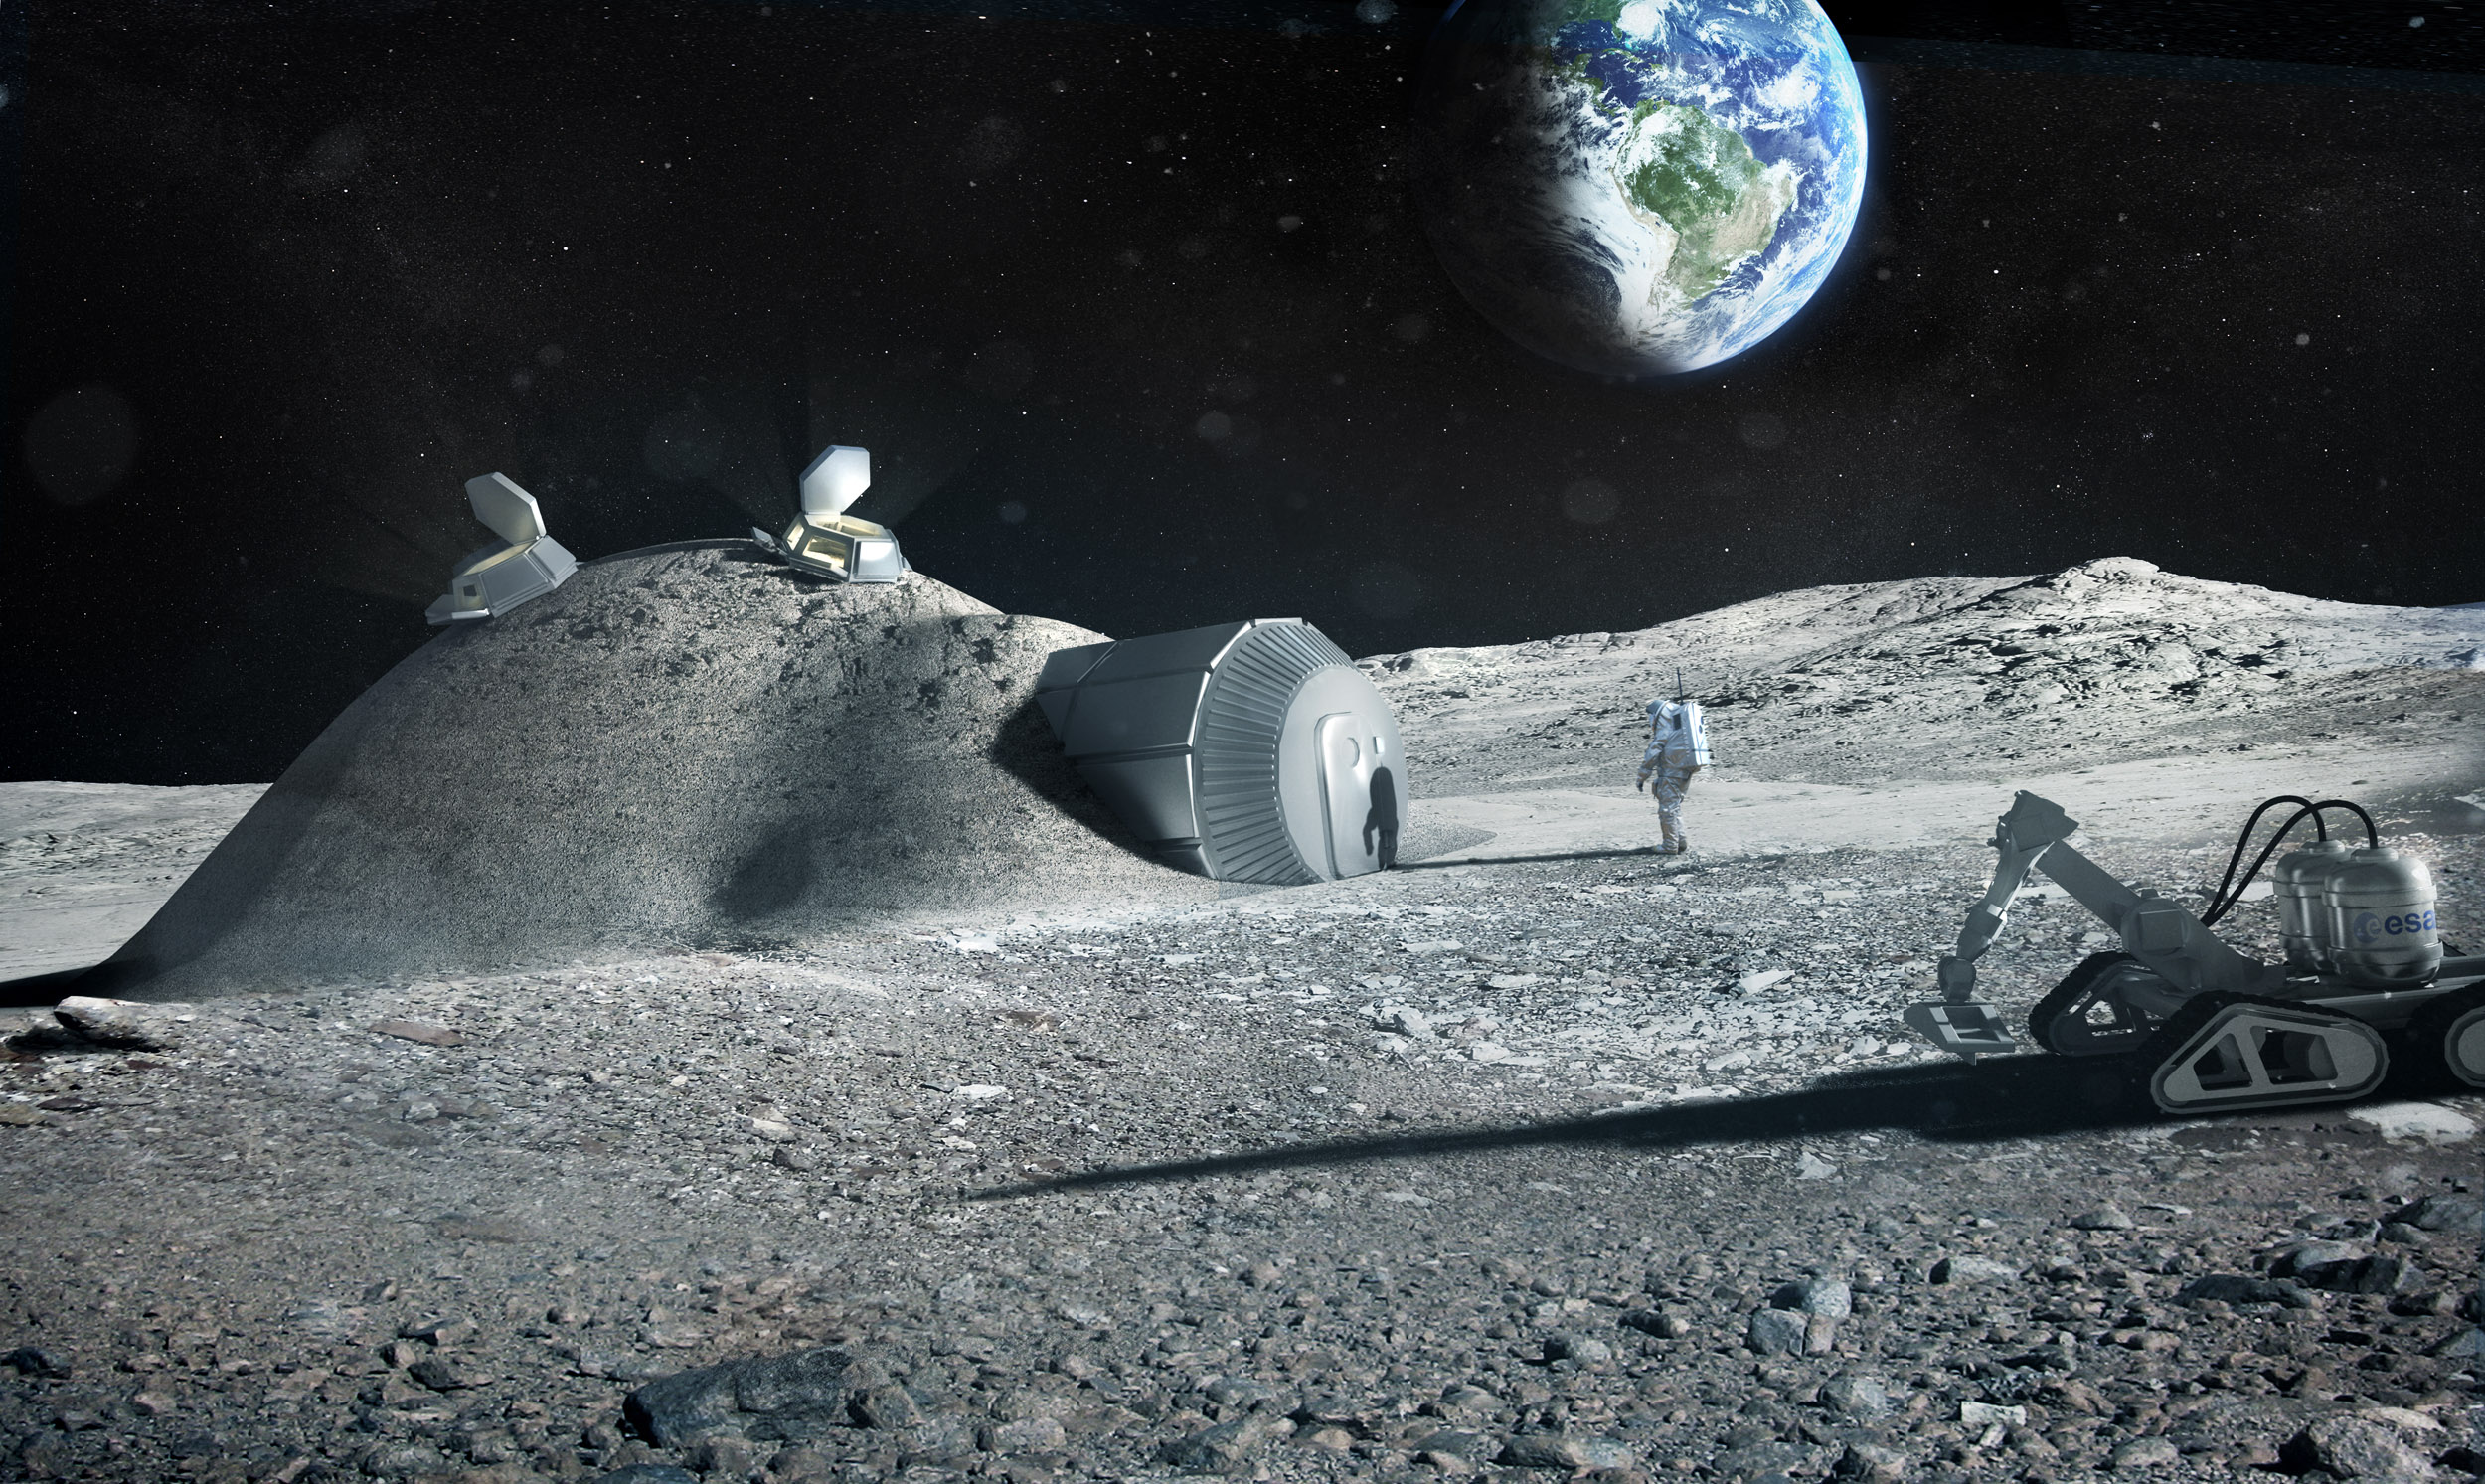
\includegraphics[height = 5cm]{../images/presentation/LunarBaseESA.jpg}
	   	\caption{Quelle: http://www.esa.int/spaceinimages/Images}
	\end{figure}
	
	%Lunar base aus 3D-Druck-Teilen und Mondgestein,
	%ESA (European Space Ageny)-Projekt,
	%Eurobot 2017-Wettbewerb unter diesem Moto

\end{frame} 

\begin{frame}
	\frametitle{Projektteam}
	
	\begin{figure}
		\begin{tikzpicture}[scale=0.5, transform shape]
		%Joel
		\def\xPos{2};	\def\yPos{1};
		\draw [draw=none, fill=hsrBlue] (\xPos - 2,\yPos - 4) rectangle (\xPos + 2,\yPos + 1);
		\draw [white] (\xPos,\yPos + 0.5) node{Joel Stolz};
		\draw [white] (\xPos,\yPos) node{\textbf{Mechanik}};
		\node[inner sep=0, outer sep=0, align=center] at (\xPos, \yPos - 2.2) {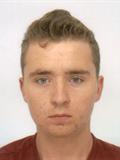
\includegraphics[height=3.5cm]{../images/Projektorganisation/joelStolz.jpg}};
		%Tibor
		\def\xPos{7};	\def\yPos{1};
		\draw [draw=none, fill=hsrBlue] (\xPos - 2,\yPos - 4) rectangle (\xPos + 2,\yPos + 1);
		\draw [white] (\xPos,\yPos + 0.5) node{Tibor Schneider};
		\draw [white] (\xPos,\yPos - 0) node{\textbf{Elektronik}};
		\node[inner sep=0, outer sep=0, align=center] at (\xPos, \yPos - 2.2) {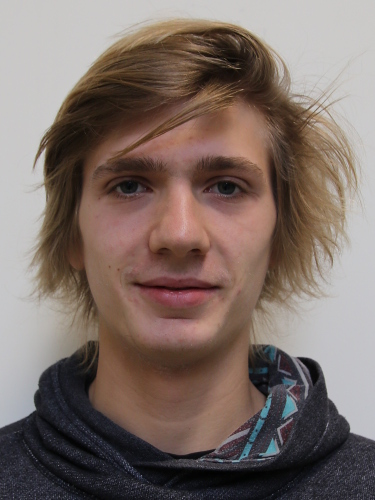
\includegraphics[height=3.5cm]{../images/Projektorganisation/tiborSchneider.jpg}};
		%cornel
		\def\xPos{12};	\def\yPos{1};
		\draw [draw=none, fill=hsrBlue] (\xPos - 2,\yPos - 4) rectangle (\xPos + 2,\yPos + 1);
		\draw [white] (\xPos,\yPos + 0.5) node{Cornel Angehrn};
		\draw [white] (\xPos,\yPos - 0) node{\textbf{Elektronik}};
		\node[inner sep=0, outer sep=0, align=center] at (\xPos, \yPos - 2.2) {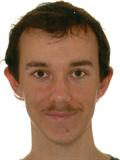
\includegraphics[height=3.5cm]{../images/Projektorganisation/cornelAngehrn.jpg}};
		%Matthias
		\def\xPos{17};	\def\yPos{1};
		\draw [draw=none, fill=hsrBlue] (\xPos - 2,\yPos - 4) rectangle (\xPos + 2,\yPos + 1);
		\draw [white] (\xPos,\yPos + 0.5) node{Matthias Knöpfel};
		\draw [white] (\xPos,\yPos - 0) node{\textbf{Elektronik}};
		\node[inner sep=0, outer sep=0, align=center] at (\xPos, \yPos - 2.2) {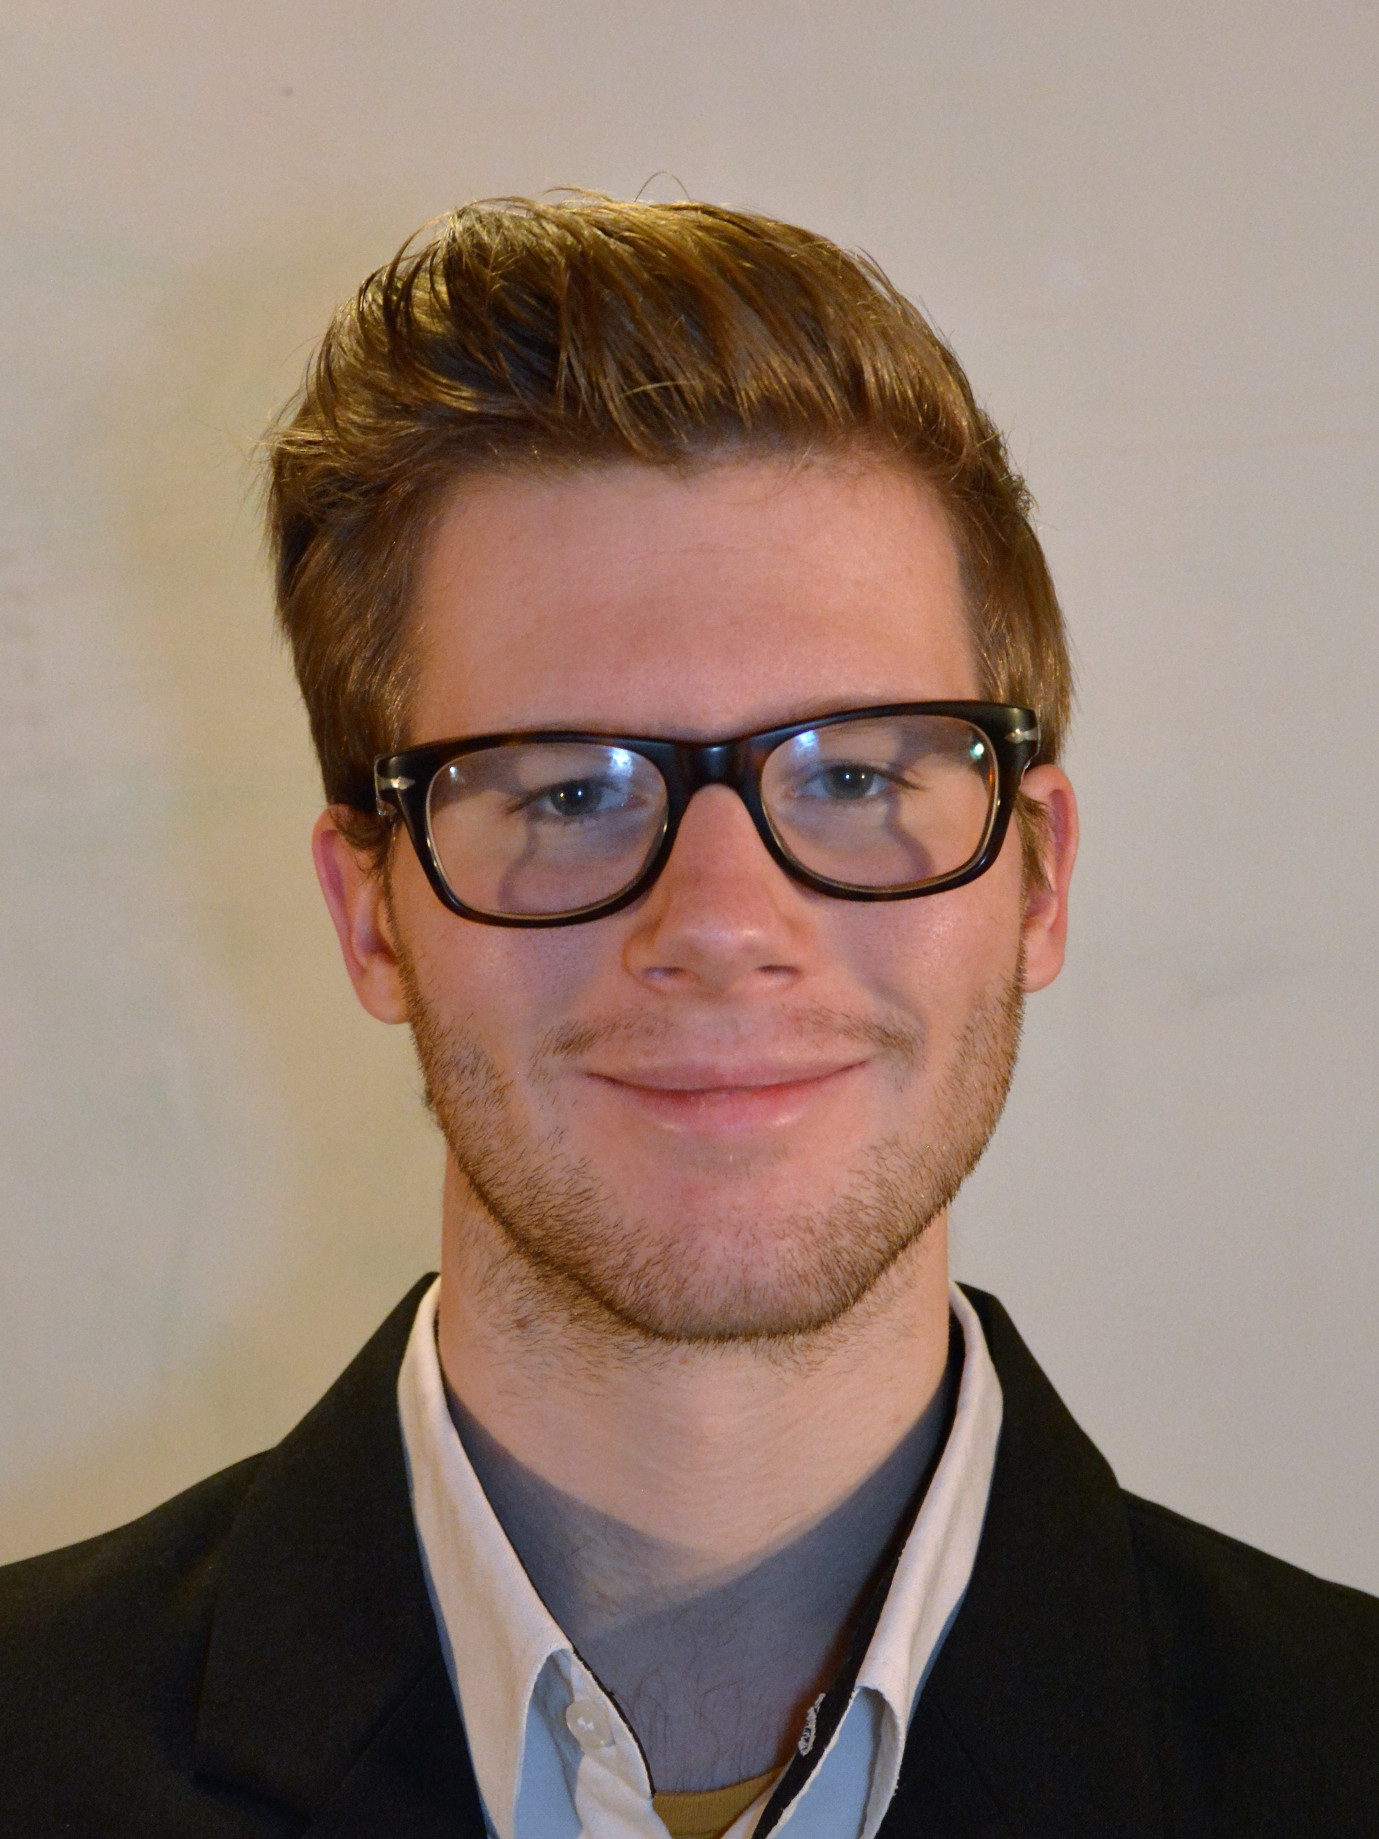
\includegraphics[height=3.5cm]{../images/Projektorganisation/matthiasKnoepfel.jpg}};
		%Petra
		\def\xPos{22};	\def\yPos{5};
		\draw [draw=none, fill=hsrBlue] (\xPos - 2,\yPos - 4) rectangle (\xPos + 2,\yPos + 1);
		\draw [white] (\xPos,\yPos + 0.5) node{Petra Freuler};
		\draw [white] (\xPos,\yPos - 0) node{\textbf{Projektleitung}};
		\node[inner sep=0, outer sep=0, align=center] at (\xPos, \yPos - 2.2) {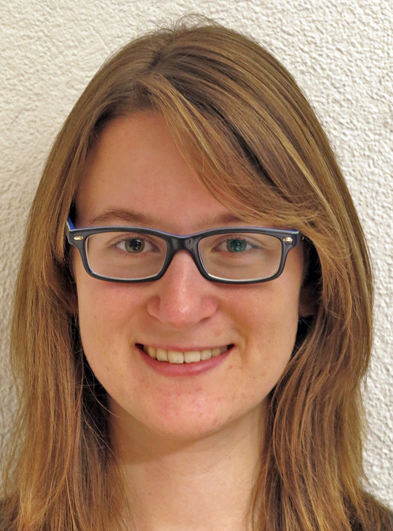
\includegraphics[height=3.5cm]{../images/Projektorganisation/petraFreuler.jpg}};
		%Wüst
		\def\xPos{2};	\def\yPos{8};
		\draw [draw=none, fill=hsrBlue] (\xPos - 2.5,\yPos - 1) rectangle (\xPos + 2.5,\yPos + 1);
		\draw [white] (\xPos,\yPos + 0.25) node{Prof. Theodor Wüst};
		\draw [white] (\xPos,\yPos - 0.25) node{\textbf{Betreuung Mechanik}};
		%Brändle
		\def\xPos{11};	\def\yPos{8};
		\draw [draw=none, fill=hsrBlue] (\xPos - 2.5,\yPos - 1) rectangle (\xPos + 2.5,\yPos + 1);
		\draw [white] (\xPos,\yPos + 0.5) node{Prof. Erwin Brändle};
		\draw [white] (\xPos,\yPos) node{\textbf{Auftraggeber}};
		\draw [white] (\xPos,\yPos - 0.5) node{\textbf{Betreuung Elektronik}};
		%Keller
		\def\xPos{17};	\def\yPos{8};
		\draw [draw=none, fill=hsrBlue] (\xPos - 2.5,\yPos - 1) rectangle (\xPos + 2.5,\yPos + 1);
		\draw [white] (\xPos,\yPos + 0.5) node{Prof. Daniel Keller};
		\draw [white] (\xPos,\yPos) node{\textbf{Betreuung}};
		\draw [white] (\xPos,\yPos - 0.5 ) node{\textbf{Projektleitung}};
		
		%connections
		\draw [thick] (2,2) -- (2,7) (2,3) -- (17,3) (7,2) -- (7,3) (12,2) -- (12,3) (17,2) -- (17,3) (11,3) -- (11,5) -- (20,5) (11,5) -- (11,7) (16,5) -- (17,5) -- (17,7);
		\end{tikzpicture}
	\end{figure}

\end{frame}

\begin{frame}
	\frametitle{Arbeitsaufteilung}
	
	\begin{itemize}
	   	\item Petra Freuler: Projektleitung %und Protokollführung
	   	\item Joel Stolz: Konstruktion, CAD	%gesamter Maschinenbauteil
	   	\item Cornel Angehrn: Gegnererkennung 
	   	\item Matthias Knöpfel: Fahrcontroller
	   	\item Tibor Schneider: Mainboard
	\end{itemize}
	
	\begin{itemize}
	   	\item Alle: Konzeptfindung, Machbarkeitstests
	\end{itemize}
	
	%Elektrotechnik: Dimensionieren und auswählen von Motoren, Sensoren und Beurteilung der Testergebnisse vorallem von elektrischer Seite (Vakuum/Saugnapf, Walze, Bälle fördern, ...)

\end{frame}
  
  %Vorgaben
  \section{Vorgaben}
\subsection{\eurobot}

\begin{frame}
	\setbeamercovered{transparent}
	\frametitle{\eurobot} % TODO besserer Titel: wie wärs mit Aufgaben?
	
	\begin{itemize}
		\item 1-2 Roboter pro Team
		\item Roboter bewegen sich autonom
		\item Behinderung und Beschädigung des Gegners ist nicht erlaubt
	\end{itemize}
	% Darum sind diverse Sensoren und die Gegnerekennung nötig
	
\end{frame}

\begin{frame}
	\frametitle{\eurobot}
	\framesubtitle{Spielfeld}
	
	\begin{figure}
	   	\centering
	   	\begin{tikzpicture}[scale=0.8, transform shape]
	   	\node[anchor=south west,inner sep=0] (image) at (0,0) {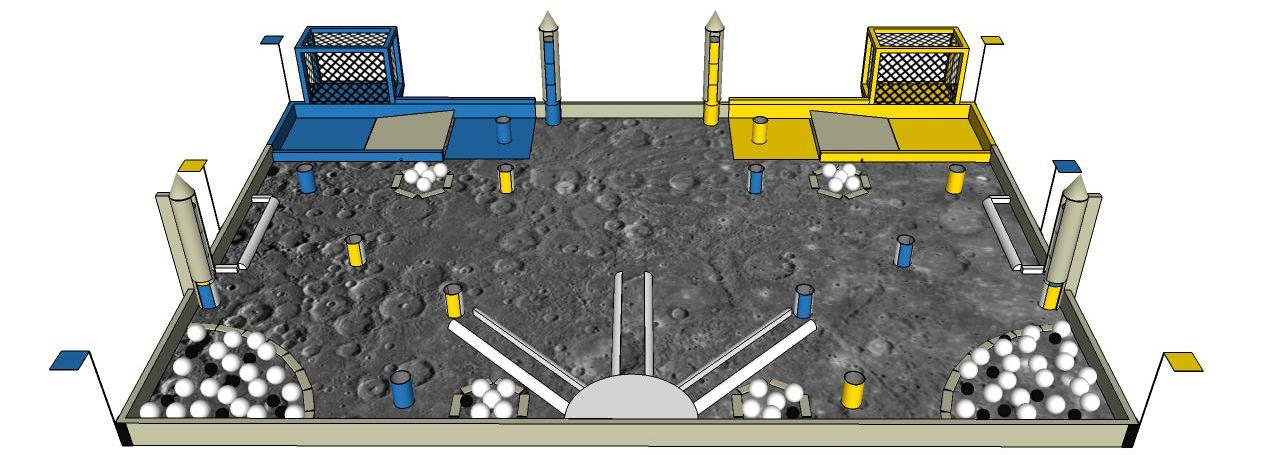
\includegraphics[width=\textwidth] {../images/spielfeldElemente.jpg}};
	   	\begin{scope}[x={(image.south east)},y={(image.north west)}]
	   	\draw [line width=0.4mm, ->, cGreen] (0.05,0.85) node[left, color=black]{\textit{cargo bay}} -- (0.235,0.85); 
	   	\draw [line width=0.4mm, ->, cGreen] (0.05,0.7) node[left, color=black]{Startfeld} -- (0.25,0.7); 
	   	\draw [line width=0.4mm, ->, cGreen] (0.05,0.55) node[left, color=black]{Rackete} -- (0.12,0.55); 
	   	\draw [line width=0.4mm, ->, cGreen] (0.05,0.4) node[left, color=black]{\textit{moon base}} -- (0.48,0.4); 
	   	\draw [line width=0.4mm, ->, cGreen] (0.05,0.25) node[left, color=black]{Krater} -- (0.14,0.25);
	   	
	   	\draw [line width=0.4mm, ->, cGreen] (0.95,0.9) node[right, color=black]{\textit{beacon}} -- (0.8, 0.9);
	   	\draw [line width=0.4mm, ->, cGreen] (0.95,0.7) node[right, color=black]{Wippe} -- (0.7, 0.7);
	   	\draw [line width=0.4mm, ->, cGreen] (0.95,0.52) node[right, color=black]{\textit{moon base}} -- (0.8, 0.52);
	   	\draw [line width=0.4mm, ->, cGreen] (0.95,0.13) node[right, color=black]{Krater} -- (0.62, 0.13);
	   	
	   	\end{scope}
	   	\end{tikzpicture}
	\end{figure}
\end{frame}

\begin{frame}
	\frametitle{\eurobot}
	\framesubtitle{\textit{Lunar Modules}}
	
	\begin{itemize}
		\item \textit{Lunar modules} seitwärts in die \textit{moon base} legen.
		\begin{itemize}
			\item mehrfarbige \textit{lunar modules} drehen, bis eigene Farbe oben ist
			% auch ins shuttle legen möglich
		\end{itemize}
	\end{itemize}

	\begin{figure}
		\begin{subfigure}{0.1\textwidth}
			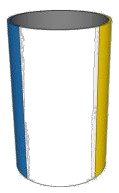
\includegraphics[width=\textwidth]{../images/lunarModuleMulticolor.jpg}
		\end{subfigure}
		\hspace{1em}
		\begin{subfigure}{0.1\textwidth}
			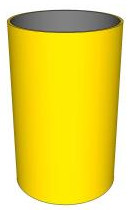
\includegraphics[width=\textwidth]{../images/lunarModule.jpg}
		\end{subfigure}
		\hspace{2em}
		\begin{subfigure}{0.5\textwidth}
			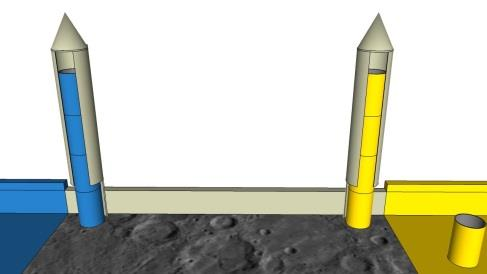
\includegraphics[width=\textwidth]{../images/rockets.jpg}
		\end{subfigure}
	\end{figure}

\end{frame}

\begin{frame}
	\frametitle{\eurobot}
	\framesubtitle{\textit{Titanium Ores}}
	
	\begin{itemize}
		\item \textit{Titanium ores} in \textit{cargo bay} befördern oder in den \textit{shuttle} legen
		% von Mondgestein trennen, da diese keine Punkte geben und im shuttle nur 10 Kugeln gezählt werden
	\end{itemize}
	
	\begin{figure}
		\begin{subfigure}{0.4\textwidth}
			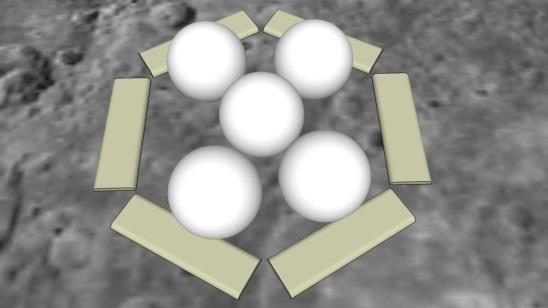
\includegraphics[height=2.5cm]{../images/craterSmall.jpg}
		\end{subfigure}
		\hspace{1em}
		\begin{subfigure}{0.4\textwidth}
			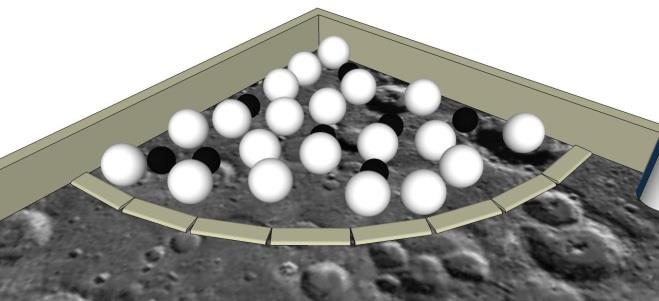
\includegraphics[height=2.5cm]{../images/craterBig.jpg}
		\end{subfigure}
	\end{figure}
	
\end{frame}


\subsection{SA-ES-350}
\begin{frame}
	\frametitle{Vorgaben SA-ES-350}
	
	\begin{itemize}
		\item Ausarbeitung der Konzepte der Roboter.
		\item Hauptkomponenten vom Vorjahr übernehmen und anpassen:
		\begin{itemize}
			\item Mainboard%: neue Hardware, Software vorbereiten
			\item Fahrcontroller%: Kurven fahren, einfachere Kalibrierung
			\item Gegnererkennung%: LED-Ring, Adapterboard, Software
		\end{itemize}
		
		\item Alle elektrischen Komponenten auswählen und bereitstellen.
	\end{itemize}

\end{frame}  

  
  %Konzepte und Lösungsansätze
  \section{Konzepte}
\subsection{Mechanik}
\begin{frame}
	\frametitle{Konzepte}
	\framesubtitle{\textit{Titanium Ores}}
	\vspace{-1em}
	\begin{figure}		
		\begin{tikzpicture}[scale=1, transform shape]
		\def\height{4.5cm}
		\node[anchor=south west,inner sep=0] (image) at (0,0) {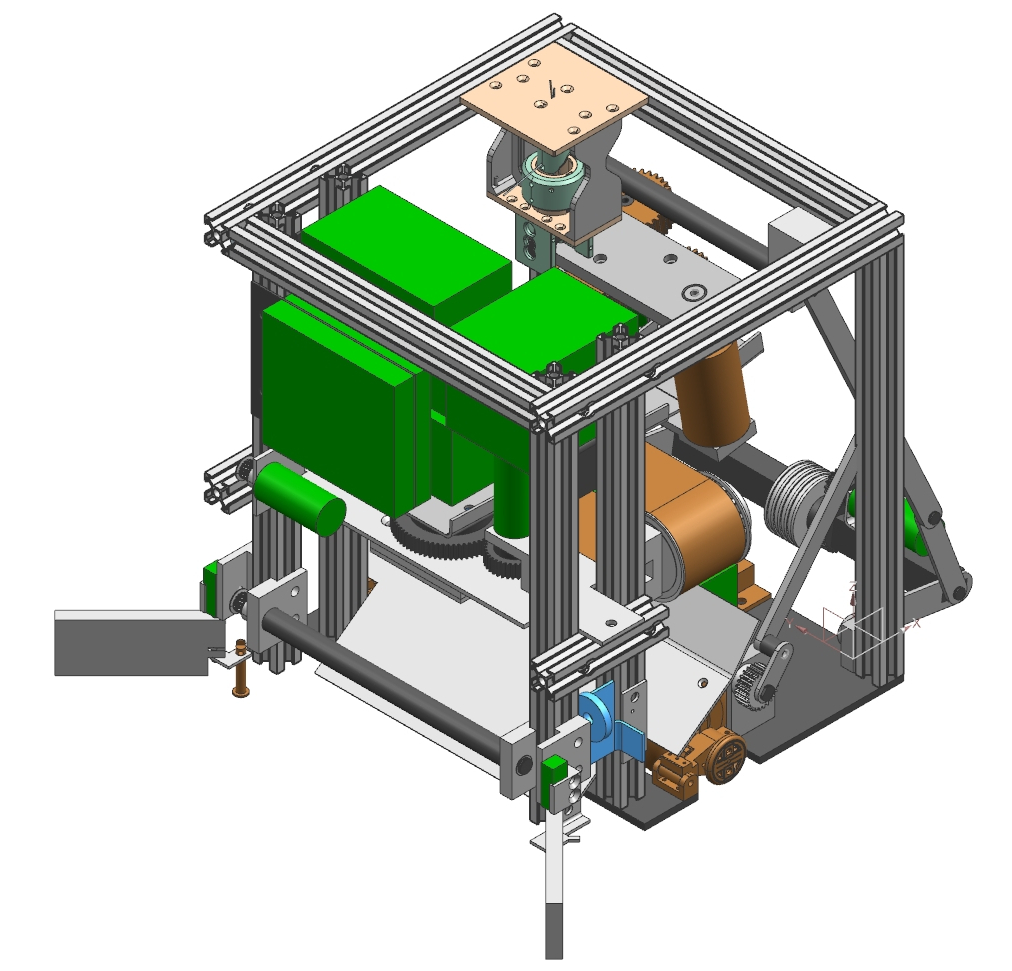
\includegraphics[height=5.5cm] {../images/mechKonzept/Roboter_grossPres.jpg}};
		
		\begin{scope}[xshift=6cm]
		\node[anchor=south west,inner sep=0] (rimage) at (0,1) {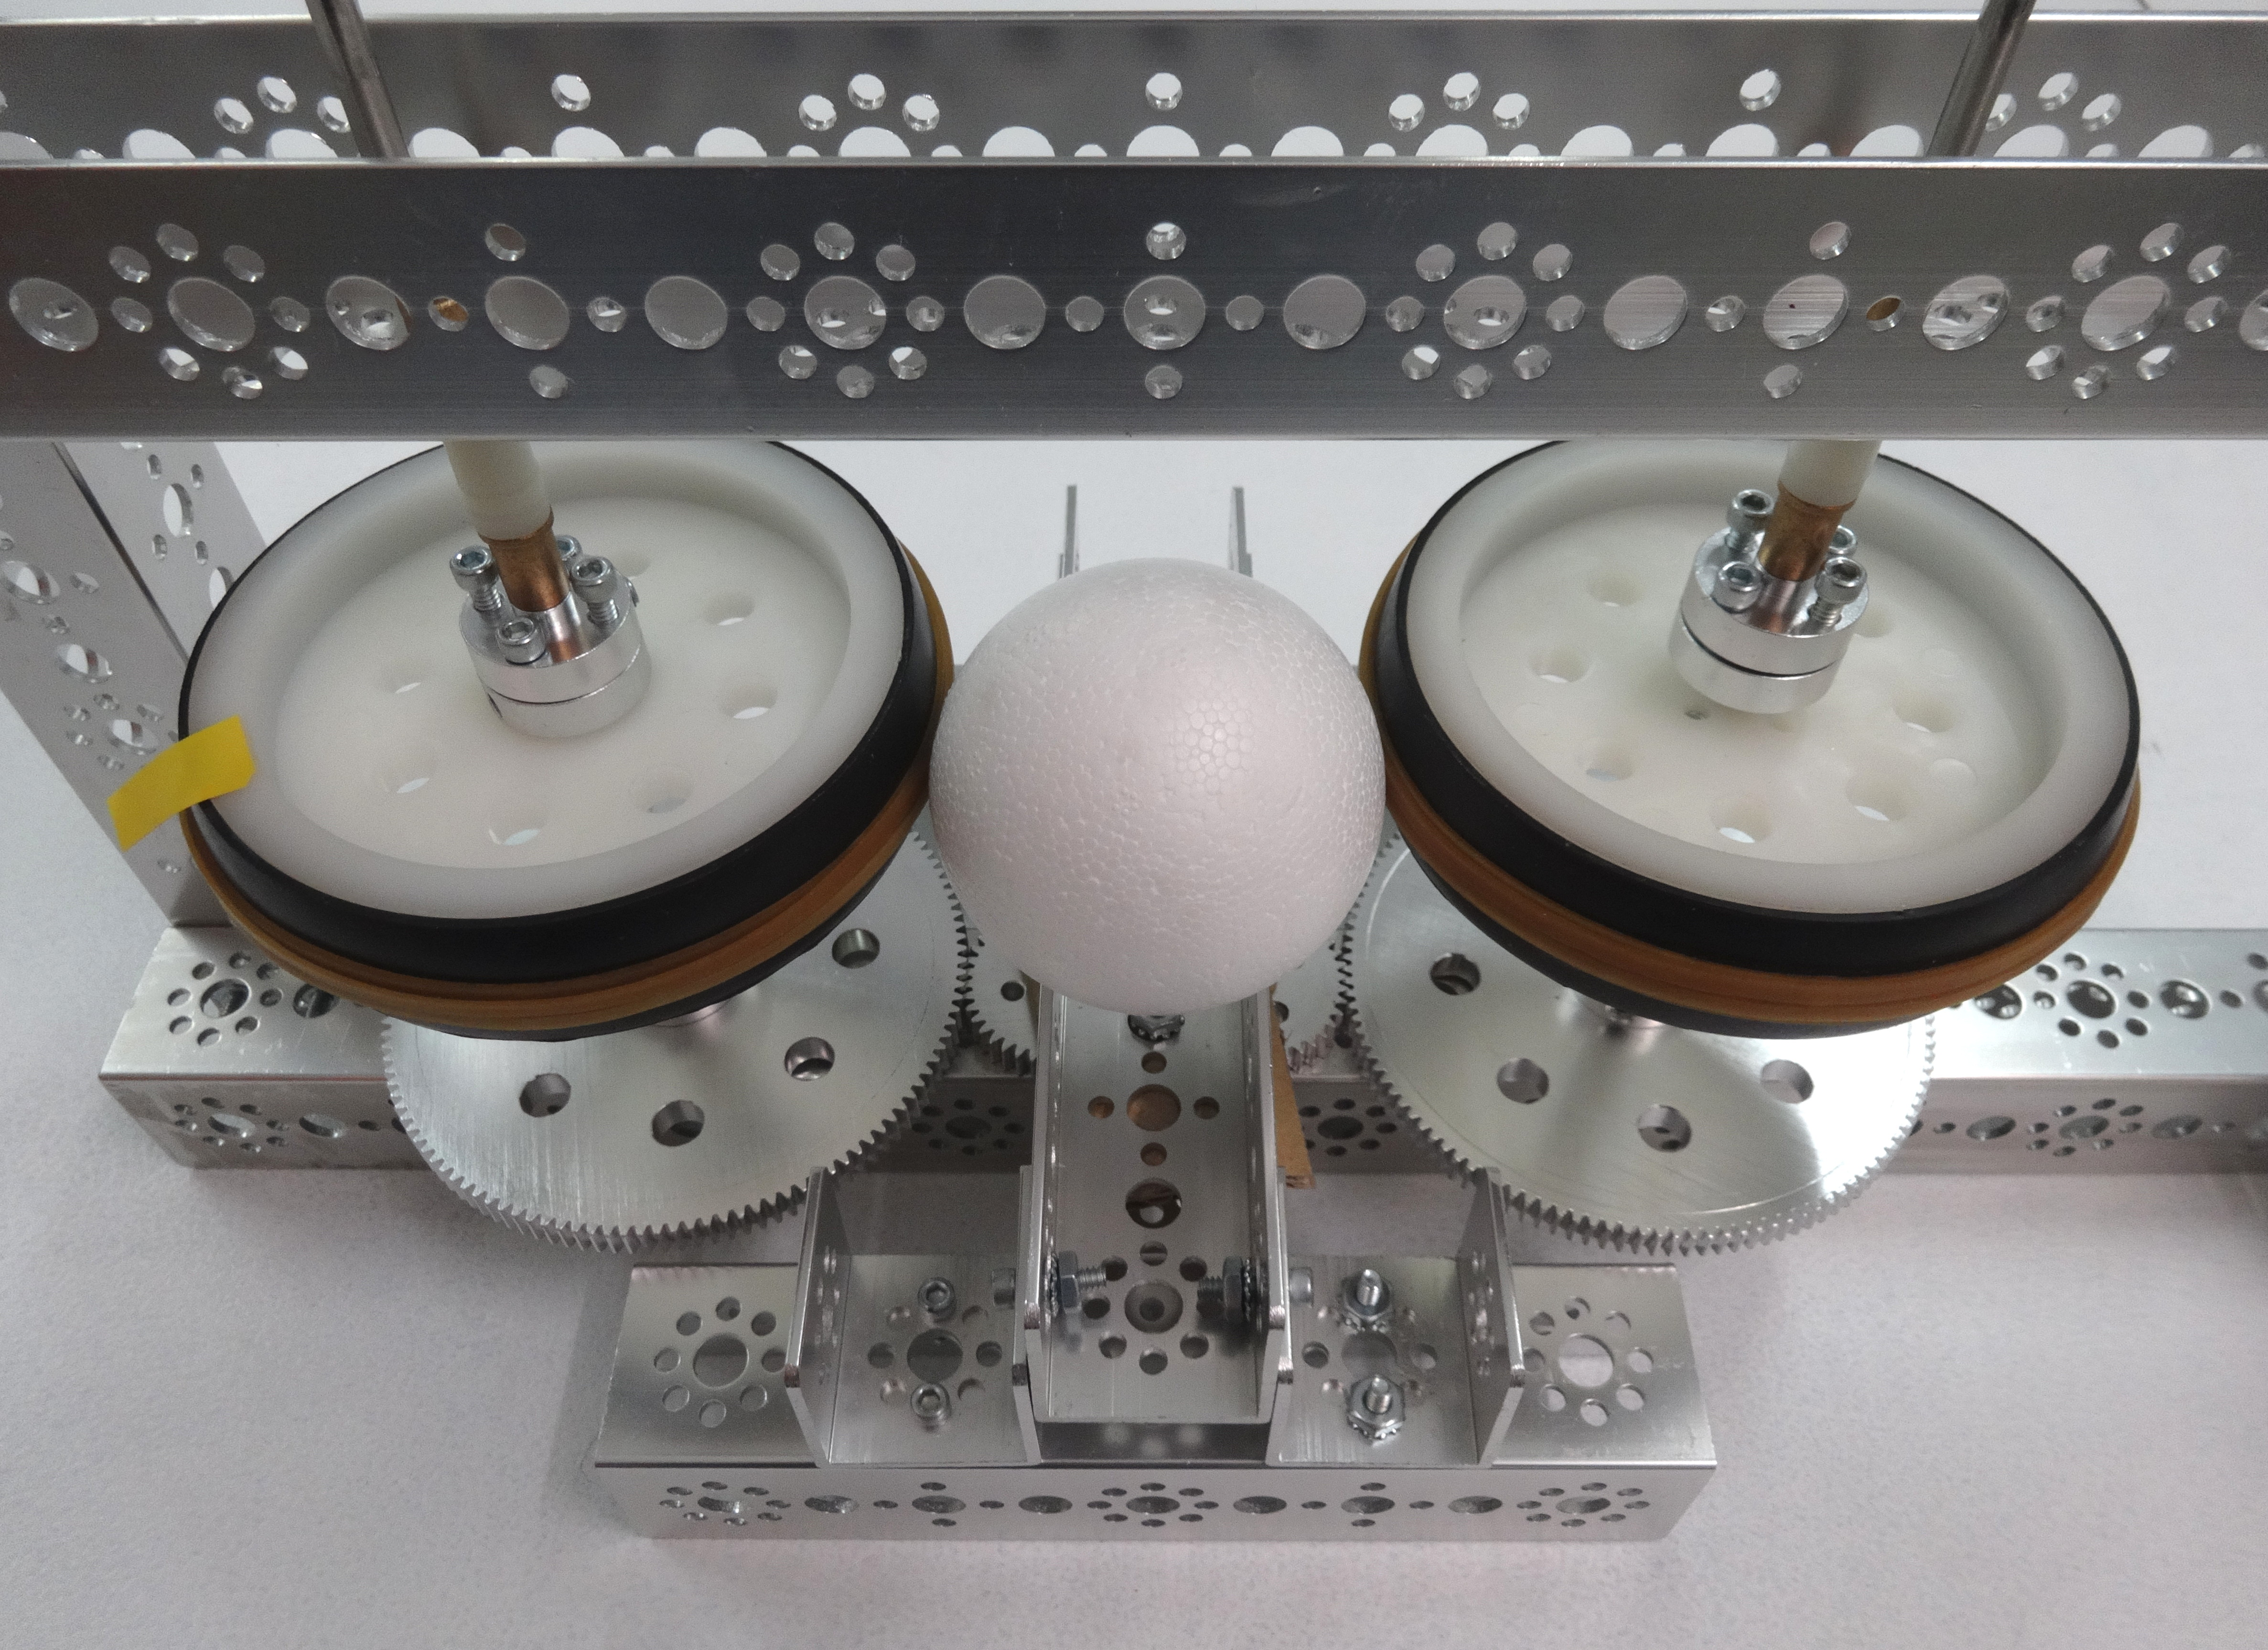
\includegraphics[height=3.5cm] {../images/mechKonzept/Ballschussanlage2.JPG}};
		
		\end{scope}
		\end{tikzpicture}	
		
		\vspace{1em}
		CAD-Modell grosser Roboter und Versuchsaufbau Ballschussmaschine
	\end{figure}

\end{frame}    

\begin{frame}
	\frametitle{Konzepte}
	\framesubtitle{\textit{Lunar Modules}}
	
	\begin{figure}
		\begin{tikzpicture}[scale=1, transform shape]
		\def\height{5cm}
		\node[anchor=south west,inner sep=0] (image) at (0,1) {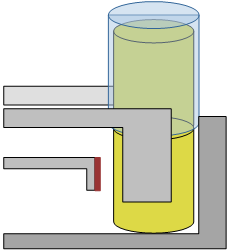
\includegraphics[height=3cm] {../images/mechKonzept/SchrankenPres.png}};
			
		\begin{scope}[xshift=4cm]
		\node[anchor=south west,inner sep=0] (rimage) at (0,0) {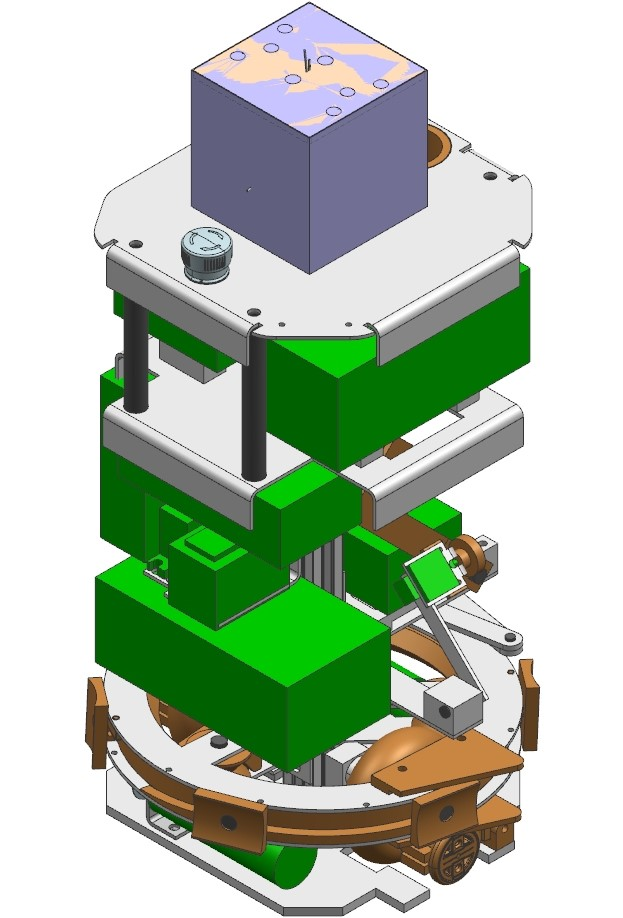
\includegraphics[height=\height] {../images/mechKonzept/Roboter_kleinPres.jpg}};
		
		\end{scope}
		\end{tikzpicture}	
		\vspace{1em}
		
		Prinzip Modulaufnahme und CAD-Modell kleiner Roboter
	\end{figure}

	  
\end{frame}

\subsection{Gesamtsystem}
\begin{frame}
	\frametitle{Elektronikmodule}
	
	\vspace{-1em}	
	\begin{figure}
		\begin{tikzpicture}[scale=0.6, every node/.style={scale=0.5}]
		% box for Robot
		\draw [color=cBlue, line width=0.6mm, rounded corners=2pt] (-2,15) node[below right]{\Large Roboter} rectangle (16,4.5);
		
		% box for Mainboard
		\draw [color=cGreen, line width = 0.4mm, rounded corners = 2pt] (4,12) rectangle (7, 10) node[pos=0.5, color=black]{\Large Mainboard};
		
		% box für Drive Controller
		\draw [color=cGreen, line width = 0.4mm, rounded corners = 2pt] (3,8) rectangle (6,6) node[pos=0.5, text width = 2.5cm, align=center, color=black] {\Large Drive \\ Controller \\ (DC)};
		
		% box für Oponent Detection
		\draw [color=cGreen, line width = 0.4mm, rounded corners = 2pt] (7,8) rectangle (10,6) node[pos=0.5, text width = 2.5cm, align=center, color=black] {\Large Oponent \\ Detection \\ (OD)};
		
		% draw CAN bus
		\draw [line width = 0.8mm] (5.5,10) -- (5.5,9) (2.5,9) node[above right] {CAN Bus} -- (11.5,9) (4.5,9) -- (4.5,8) (8.5,9) -- (8.5,8);
		
		%draw Display
		\draw [line width = 0.4mm, color = cRed, rounded corners = 2pt] (9,14.5) rectangle (12,13.5) node[pos=0.5, color=black] {\Large Display};
		\draw [line width = 0.4mm, rounded corners = 2pt] (6,12) -- (6,14) node[above right]{SPI} -- (9,14);
		
		%draw Bluetooth
		\draw [line width = 0.4mm, color = cRed, rounded corners = 2pt] (9,13) rectangle (12,12) node[pos=0.5, color=black] {\Large Bluetooth};
		\draw [line width = 0.4mm, rounded corners = 2pt] (6.5,12) -- (6.5,12.5) node[above right]{UART} -- (9,12.5);
		
		%draw Datenlogger
		\draw [line width = 0.4mm, color = cRed, rounded corners = 2pt] (9,11.5) rectangle (12,10.5) node[pos=0.5, color=black] {\Large Datenlogger};
		\draw [line width = 0.4mm, rounded corners = 2pt] (7,11) node[above right]{UART} -- (9,11);
		
		%draw Powerboard
		\draw [line width = 0.4mm, color=cGreen, rounded corners = 2pt] (2,14.5) rectangle (5,13) node[pos=0.5, color=black] {\Large Powerboard};
		\draw [line width = 0.4mm, rounded corners = 2pt] (2.5,13) -- (2.5,11) node[above right] {Direkt} -- (4,11);
		
		%draw LED ring
		\draw [line width = 0.4mm, color = cRed, rounded corners = 2pt] (12.4,7.5) rectangle (15.5,8.5) node[pos=0.5, color=black] {\Large LED Ring};
		\draw [line width = 0.4mm, rounded corners = 2pt] (10,7.5) -- (10.5,7.5) -- (10.5,8) node[above right]{SPI} -- (12.4,8);
		
		%draw OD motoren und sensoren
		\draw [line width = 0.4mm, color = cRed, rounded corners = 2pt] (12.4,6) rectangle (15.5,7) node[pos=0.5, color=black] {\Large Motor, Sensoren};
		\draw [line width = 0.4mm, rounded corners = 2pt] (10,6.5) node[above right]{Direkt} -- (12.4,6.5);
		
		%draw 9 achsen sensor
		\draw [line width = 0.4mm, color = cRed, rounded corners = 2pt] (-1.5,8) rectangle (1.6,9) node[pos=0.5, color=black] {\Large 9-Achsen Sensor};
		\draw [line width = 0.4mm, rounded corners = 2pt](1.6,8.5) node[below right, xshift=0.5cm]{I$^2$C}-- (4,8.5) -- (4,8);
		
		%Schleppräder
		\draw [line width = 0.4mm, color = cRed, rounded corners = 2pt] (-1.5,7.5) rectangle (1.6,6.5) node[pos=0.5, color=black] {\Large Schleppräder};
		\draw [line width = 0.4mm, rounded corners = 2pt] (1.6,7) -- (3,7) node[below left]{SPI};
		
		%Motoren
		\draw [line width = 0.4mm, color = cRed, rounded corners = 2pt] (-1.5,6) rectangle (1.6,5) node[pos=0.5, color=black] {\Large Motoren};
		\draw [line width = 0.4mm, rounded corners = 2pt] (1.6,5.5) -- (4,5.5) node[below left]{PWM} -- (4,6);
		
		\end{tikzpicture}
	\end{figure}

\end{frame}

\begin{frame}
	\frametitle{Sensoren und Aktoren}
	
	\begin{itemize}
		\item Diverse Motoren, Servoantriebe und Sensoren nötig
		\item Wenn möglich Servos vorgesehen %Intelligente Servos, normale Servos, DC-Motoren für grössere Drehbereiche und wo Kraft nötig ist
		\item Sensoren: nur Farbsensor zur Erkennung Modulfarbe ausgewählt
	\end{itemize}   

	\begin{figure}
		\captionsetup[subfigure]{font=scriptsize,labelfont=scriptsize}
		\begin{subfigure}{0.2\textwidth}
			\centering
			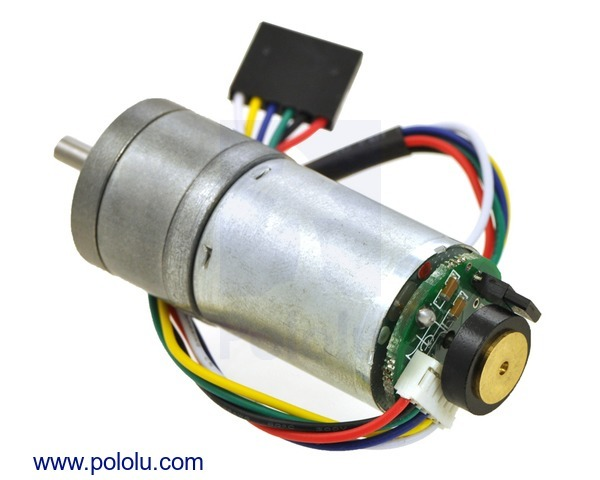
\includegraphics[height=2cm] {../images/presentation/DCMotor.jpg}
			\subcaption*{Quelle: popolu.com}
		\end{subfigure}
		\hspace{1em}
		\begin{subfigure}{0.2\textwidth}
			\centering
			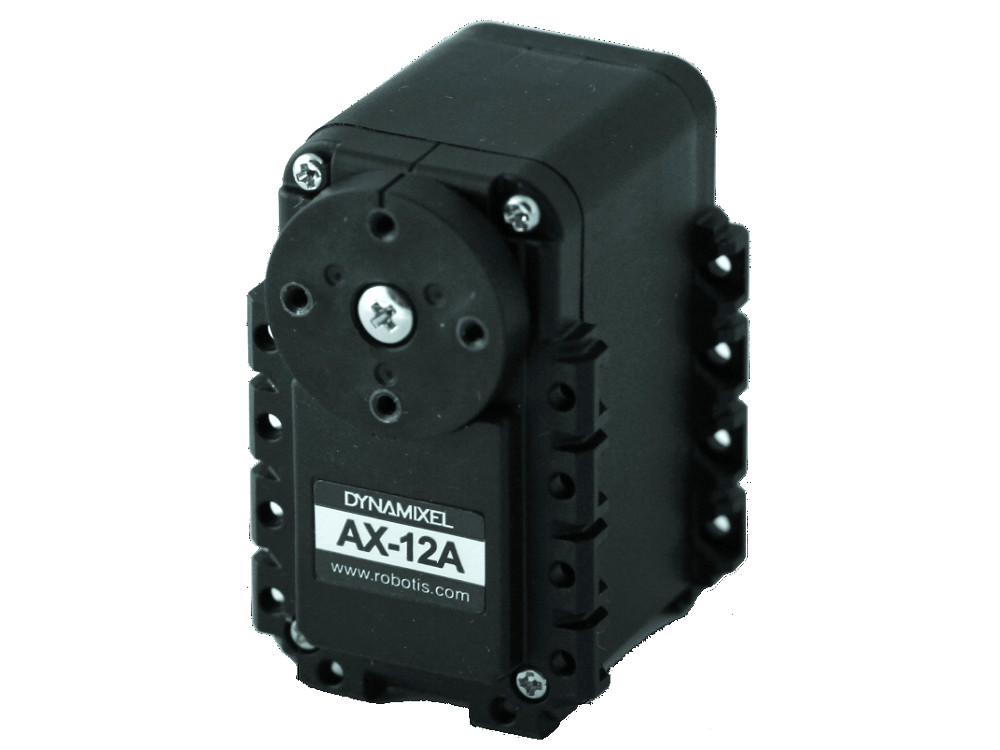
\includegraphics[height=2cm] {../images/presentation/IntServo.jpg}
			\subcaption*{Quelle: diigiit.com}
		\end{subfigure}
		\hspace{1em}
		\begin{subfigure}{0.2\textwidth}
			\centering
			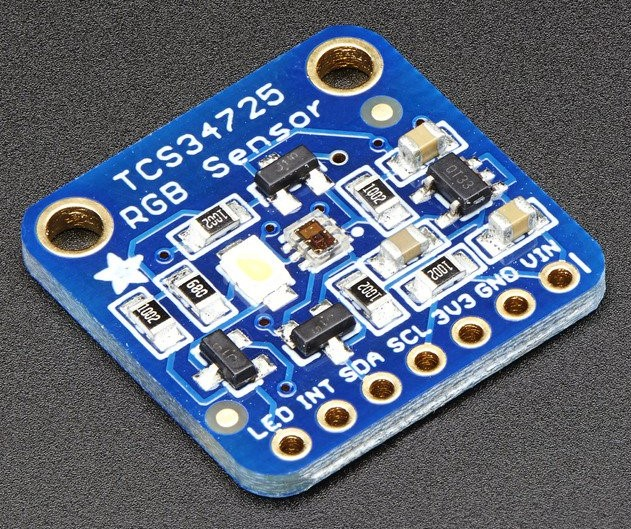
\includegraphics[height=2cm] {../images/presentation/RGB.jpg}
			\subcaption*{Quelle: adafruit.com}
		\end{subfigure}
		\hspace{1em}
	\end{figure}
	
	%Quelle: https://cdn-shop.adafruit.com/970x728/1334-04.jpg
	%Quelle: https://a.pololu-files.com/picture/0J3799.600x480.jpg?03a71976857bd4e6d447a7cd8817f31c
	%Quelle: http://www.eu.diigiit.com/dynamixel-ax-12a
\end{frame}
  
  %Mainboard
  \section{Mainboard}

\begin{frame}
	\setbeamercovered{transparent}
	\frametitle{Mainboard}
	
	\begin{columns}
		\begin{column}{0.5\textwidth}
			\begin{itemize}
				\item Neue Hardware
				\item Neue oder überarbeitete Module:
				\begin{itemize}
					\item Bluetooth Kommunikation
					\item Display
					\item CAN Kommunikation
				\end{itemize}
			\end{itemize}
		\end{column}
	
		\begin{column}{0.5\textwidth}
			\begin{figure}
				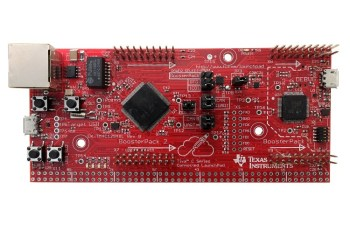
\includegraphics[width=0.8\textwidth]{../images/tiva_tm4c1294xl_ek.jpg}
			\end{figure}
		\end{column}
	\end{columns}
\end{frame}

\begin{frame}
	\frametitle{Mainboard}
	\framesubtitle{Bluetooth Kommunikation}
	
	\begin{tikzpicture}[scale=0.7, transform shape]
		%grosser roboter 
		
		%mainboard
		\draw[thick] (0.5,0.5) coordinate (big mb) rectangle ++(3,2) node[pos=0.5, align=center]{Mainboard\\Grosser Roboter}; 
		\draw (big mb) ++ (3,1) coordinate (big mb uart);
		%btDongle
		\draw[thick] (5,1) coordinate (big bt) rectangle ++(2,1) node[pos=0.5]{Bluetooth};
		\draw (big bt) ++ (0,0.5) coordinate (big bt uart);
		\draw (big bt) ++ (2,0.5) coordinate (big bt bt);
		\draw (big bt bt) -- ++ (0.5,0) -- ++ (0,1) circle (0.1) coordinate (big bt antenna);
		\foreach \r in {.2,.3,.4}
		\draw (big bt antenna) ++ (60:\r) arc (60:-60:\r);
		
		%kleiner Roboter
		%btDongle
		\draw[thick] (10.5,1) coordinate (small bt) rectangle ++(2,1) node[pos=0.5]{Bluetooth};
		\draw (small bt) ++ (2,0.5) coordinate (small bt uart);
		\draw (small bt) ++ (0,0.5) coordinate (small bt bt);
		\draw (small bt bt) -- ++ (-0.5,0) -- ++ (0,1) circle (0.1) coordinate (small bt antenna);
		\foreach \r in {.2,.3,.4}
		\draw (small bt antenna) ++ (120:\r) arc (120:240:\r);
		%mainboard
		\draw[thick] (14,0.5) coordinate (small mb) rectangle ++(3,2) node[pos=0.5, align=center]{Mainboard\\Kleiner Roboter}; 
		\draw (small mb) ++ (0,1) coordinate (small mb uart);
		
		%connections
		\draw (big mb uart) -- (big bt uart) node [pos=0.5, above] {UART};
		\draw (small mb uart) -- (small bt uart) node [pos=0.5, above] {UART};
	
	\end{tikzpicture}
	
\end{frame}

\begin{frame}
	\setbeamercovered{invisible}
	\frametitle{Mainboard}
	\framesubtitle{Bluetooth Kommunikation}
	
	\begin{figure}
		\begin{tikzpicture} [y=-1cm, scale=0.75, transform shape]
		\draw [thick] (-1.5,-1.5) rectangle ++(3,1.5) node[pos=0.5, align=center]{Grosser Roboter \\\footnotesize Master};
		\draw [thick] (4.5,-1.5) rectangle ++(3,1.5) node[pos=0.5, align=center]{Kleiner Roboter\\\footnotesize Slave};
		\draw [->] (0,0) -- ++(0,6.5) node[above right]{Zeit};
		\draw [->] (6,0) -- ++(0,6.5);
		\uncover<2>{
			\draw[thick, cRed, ->] (6,0.5) -- (0,1.5);
			\draw[fill=clRed!60!white, draw=cRed] (4.5,0.75) ++ (-0.8,-0.4) rectangle ++(1.6,0.8) node[pos=0.5, align=center]{\lstinline|msg|};
			\draw [thick, cRed, ->] (0,5) -- (6,6);
			\draw [fill=clRed!60!white, draw=cRed] (1.5,5.25) ++ (-0.8,-0.4) rectangle ++(1.6,0.8) node[pos=0.5, align=center]{\lstinline|ack|};
			\draw [thick, dotted, rounded corners=0.4cm, cRed] (0,1.5) -- (-0.5,1.5) -- (-0.5,5) -- (0,5);
		}
		\draw [thick, cGreen, ->] (0,1) -- (6,2);
		\draw [fill=clGreen!60!white, draw=cGreen] (1.5,1.25) ++ (-0.8,-0.4) rectangle ++(1.6,0.8) node[pos=0.5, align=center]{\lstinline|req|};
		\draw [thick, cGreen, ->] (6,2.5) -- (0,3.5);
		\draw [fill=clGreen!60!white, draw=cGreen] (4.5,2.75) ++ (-0.8,-0.4) rectangle ++(1.6,0.8) node[pos=0.5, align=center]{\lstinline|ans|};
		\draw [thick, cGreen, ->] (0,4) -- (6,5);
		\draw [fill=clGreen!60!white, draw=cGreen] (1.5,4.25) ++ (-0.8,-0.4) rectangle ++(1.6,0.8) node[pos=0.5, align=center]{\lstinline|ack|};
		
		\end{tikzpicture}
	\end{figure}

	\setbeamercovered{transparent}

\end{frame}

\begin{frame}
	\frametitle{Mainboard}
	\framesubtitle{Display}
	
	\begin{columns}
		\begin{column}{0.3\textwidth}
			\begin{itemize}
				\item Konfiguration zur Laufzeit
				\item Kalibrierung
			\end{itemize}
		\end{column}
		\begin{column}{0.7\textwidth}
			\vspace{-1em}
			\begin{figure}
				\begin{subfigure}{0.4\textwidth}
					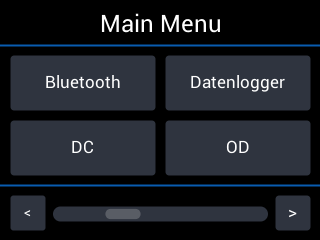
\includegraphics[width=\textwidth]{../images/displayMainMenu.png}
				\end{subfigure}
				\hspace{0.9em}
				\begin{subfigure}{0.4\textwidth}
					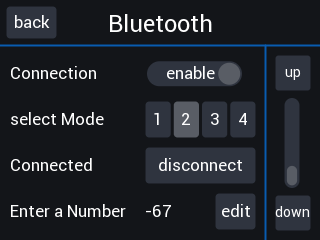
\includegraphics[width=\textwidth]{../images/displaySubMenu.png}
				\end{subfigure}
				
				\vspace{1.4em}
				\begin{subfigure}{0.4\textwidth}
					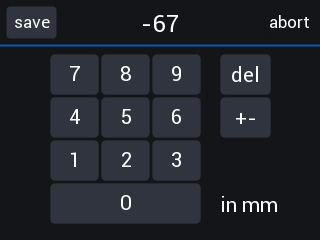
\includegraphics[width=\textwidth]{../images/displayNumberInput.png}
				\end{subfigure}
				\hspace{0.9em}
				\begin{subfigure}{0.4\textwidth}
					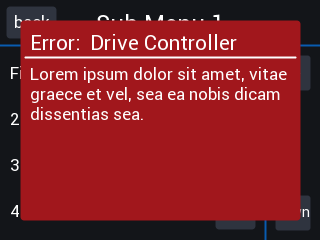
\includegraphics[width=\textwidth]{../images/displayNotification.png}
				\end{subfigure}
			\end{figure}
		\end{column}
	\end{columns}
	
\end{frame}
  
  %Gegnererkennung
  \section{Gegnererkennung}
\begin{frame}
\frametitle{Gegnererkennung}
\framesubtitle{Komponenten}

\begin{figure}
	\begin{tikzpicture}[scale=1, transform shape]
	\def\height{4cm}
	\node[anchor=south west,inner sep=0] (image) at (0,0) {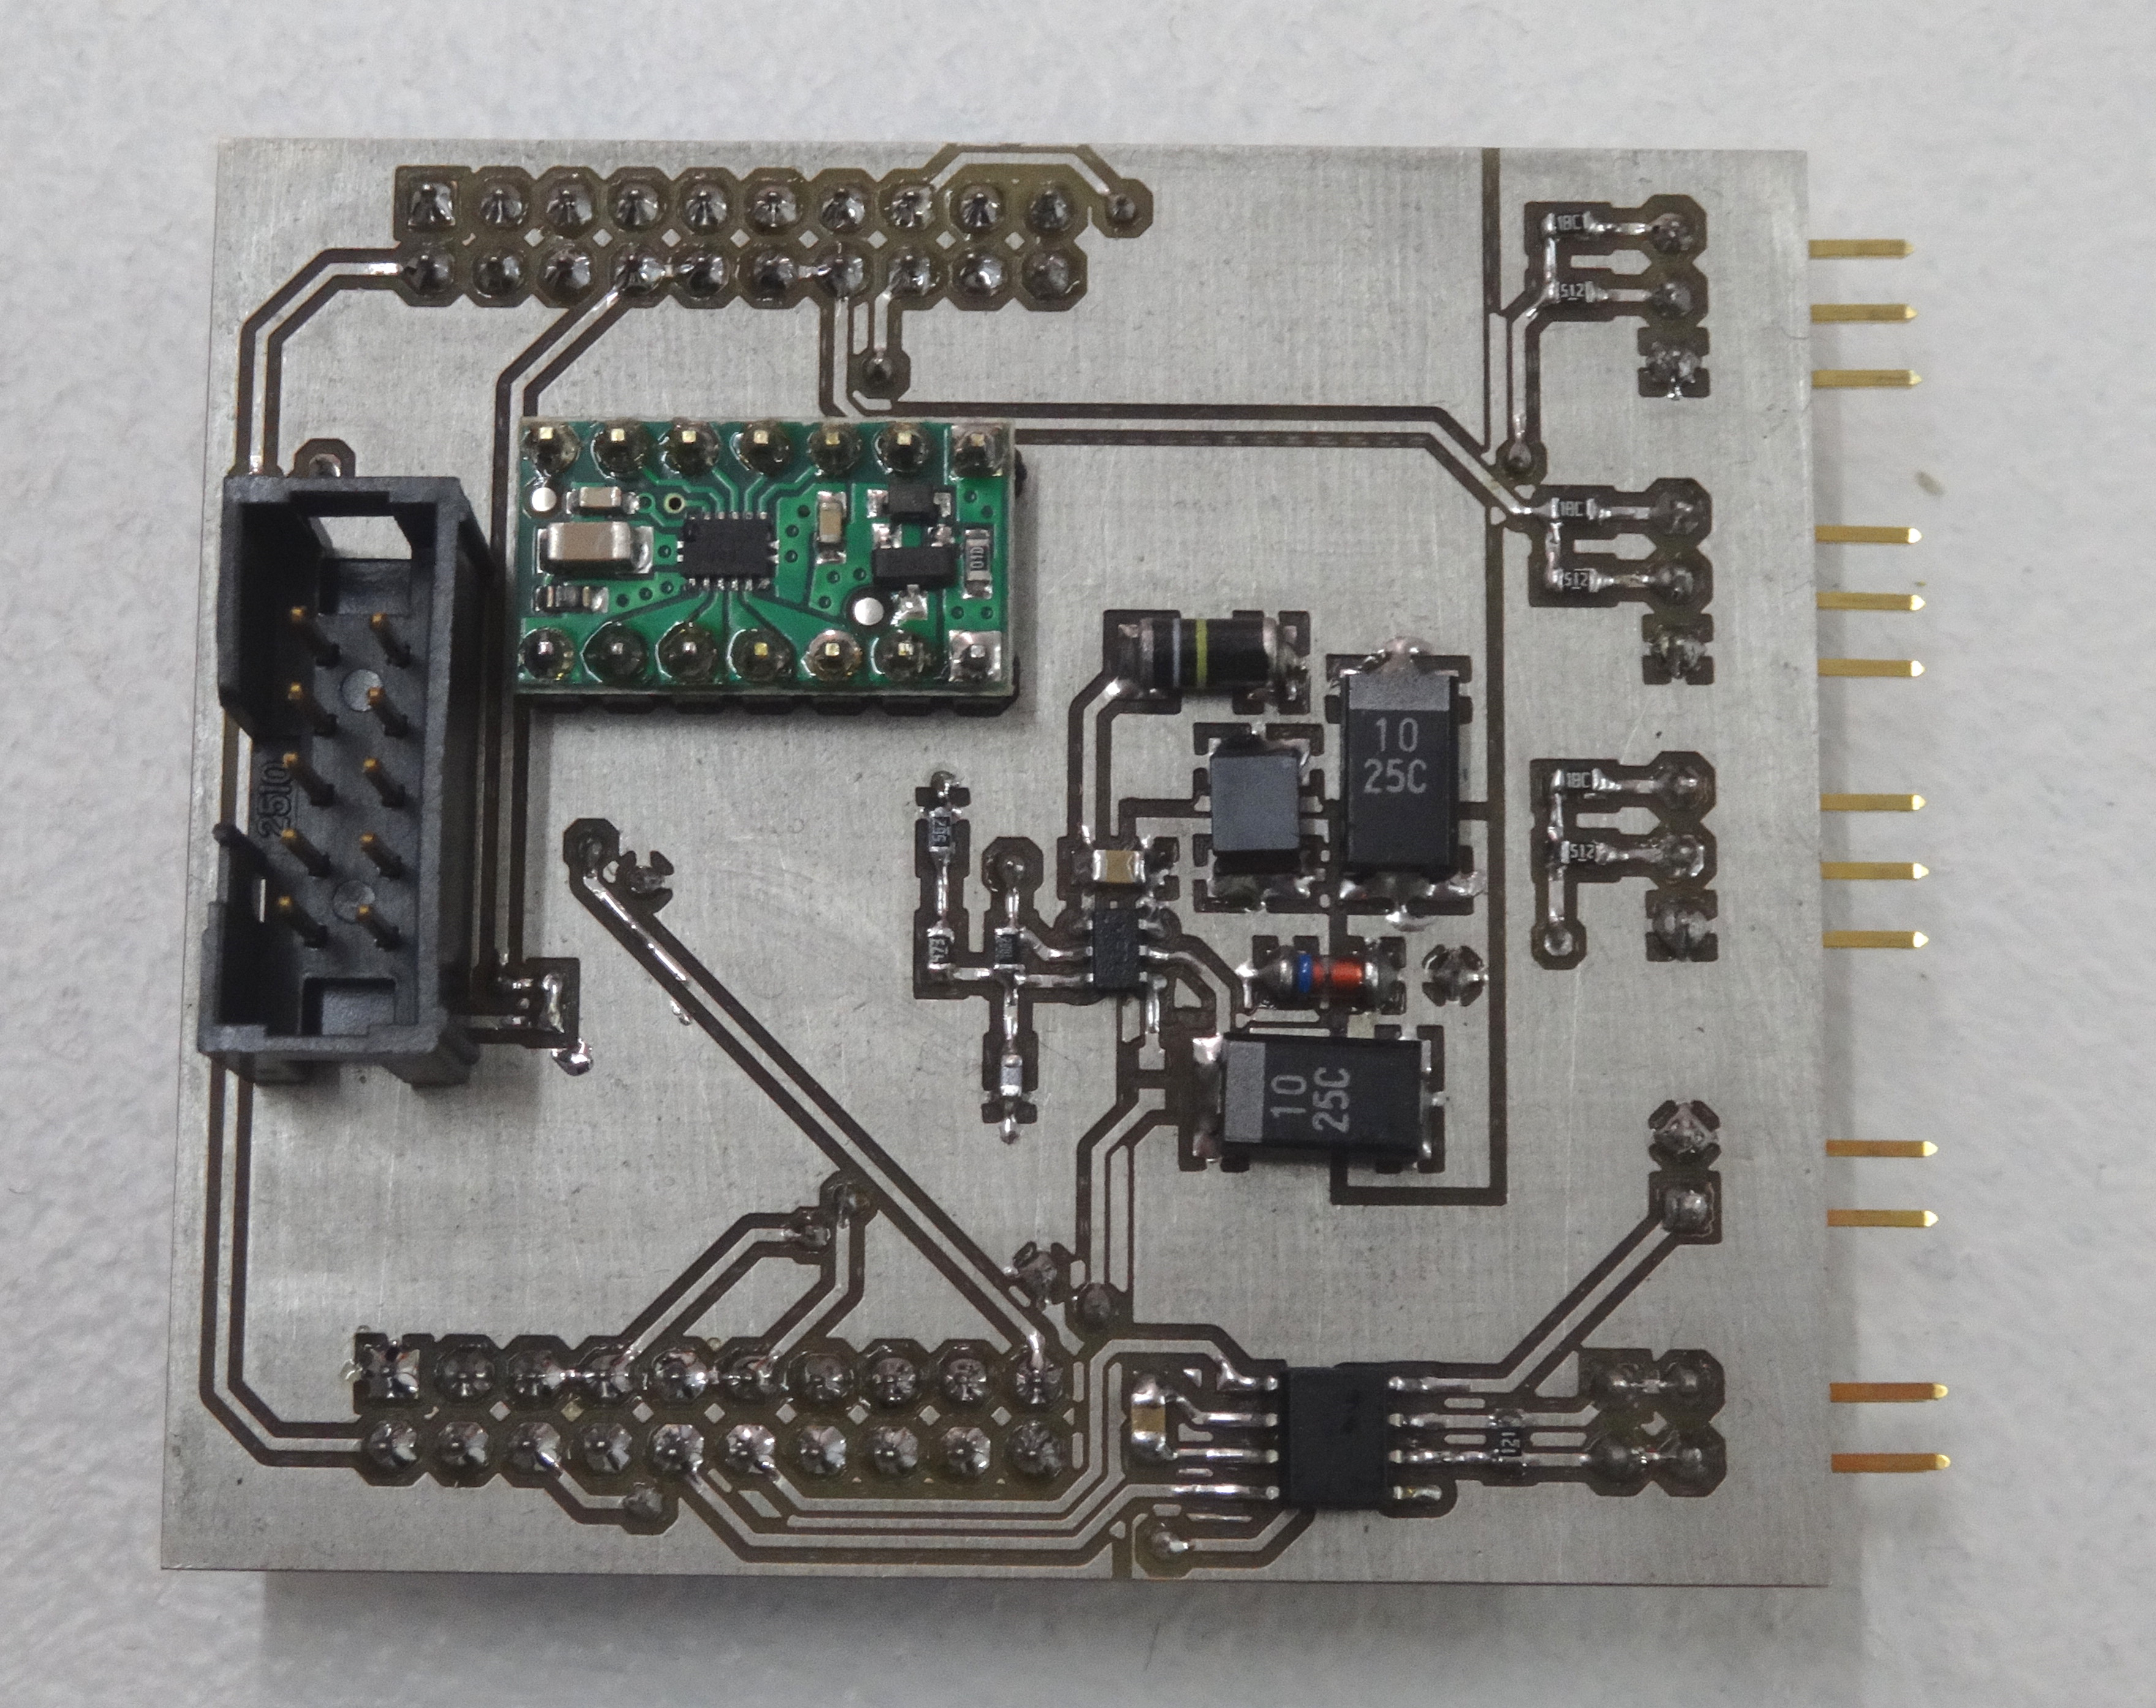
\includegraphics[height=\height] {../images/OD/Adapterboard4.JPG}};
	\begin{scope}[x={(image.south east)},y={(image.north west)}]
		\draw [line width=0.4mm, ->, cGreen] (0.35,1.1) node[left, color=black]{Treiberstufe} -- (0.35,0.75);  
		
		\draw [line width=0.4mm, ->, cGreen] (0.52,1.1) node[right, color=black]{Spannungsregler} -- (0.52, 0.5);
		\draw [line width=0.4mm, ->, cGreen] (0.62,-0.1) node[right, color=black]{CAN-Treiber} -- (0.62, 0.10);
		
		\draw [line width = 0.6mm, -, cRed] (0.15,0.5) to[out = 270, in = 180] (0.5, -0.2);
		\draw [line width = 0.6mm, -, cRed] (0.5, -0.2) -- (1.0, -0.2); 
		%\draw [line width = 0.6mm, -, cRed] (1.0, -0.2) to[out = 0, in = 270] (1.37, 0.1);
		
	\end{scope}
	
	\begin{scope}[xshift=6cm]
		\node[anchor=south west,inner sep=0] (rimage) at (0,0) {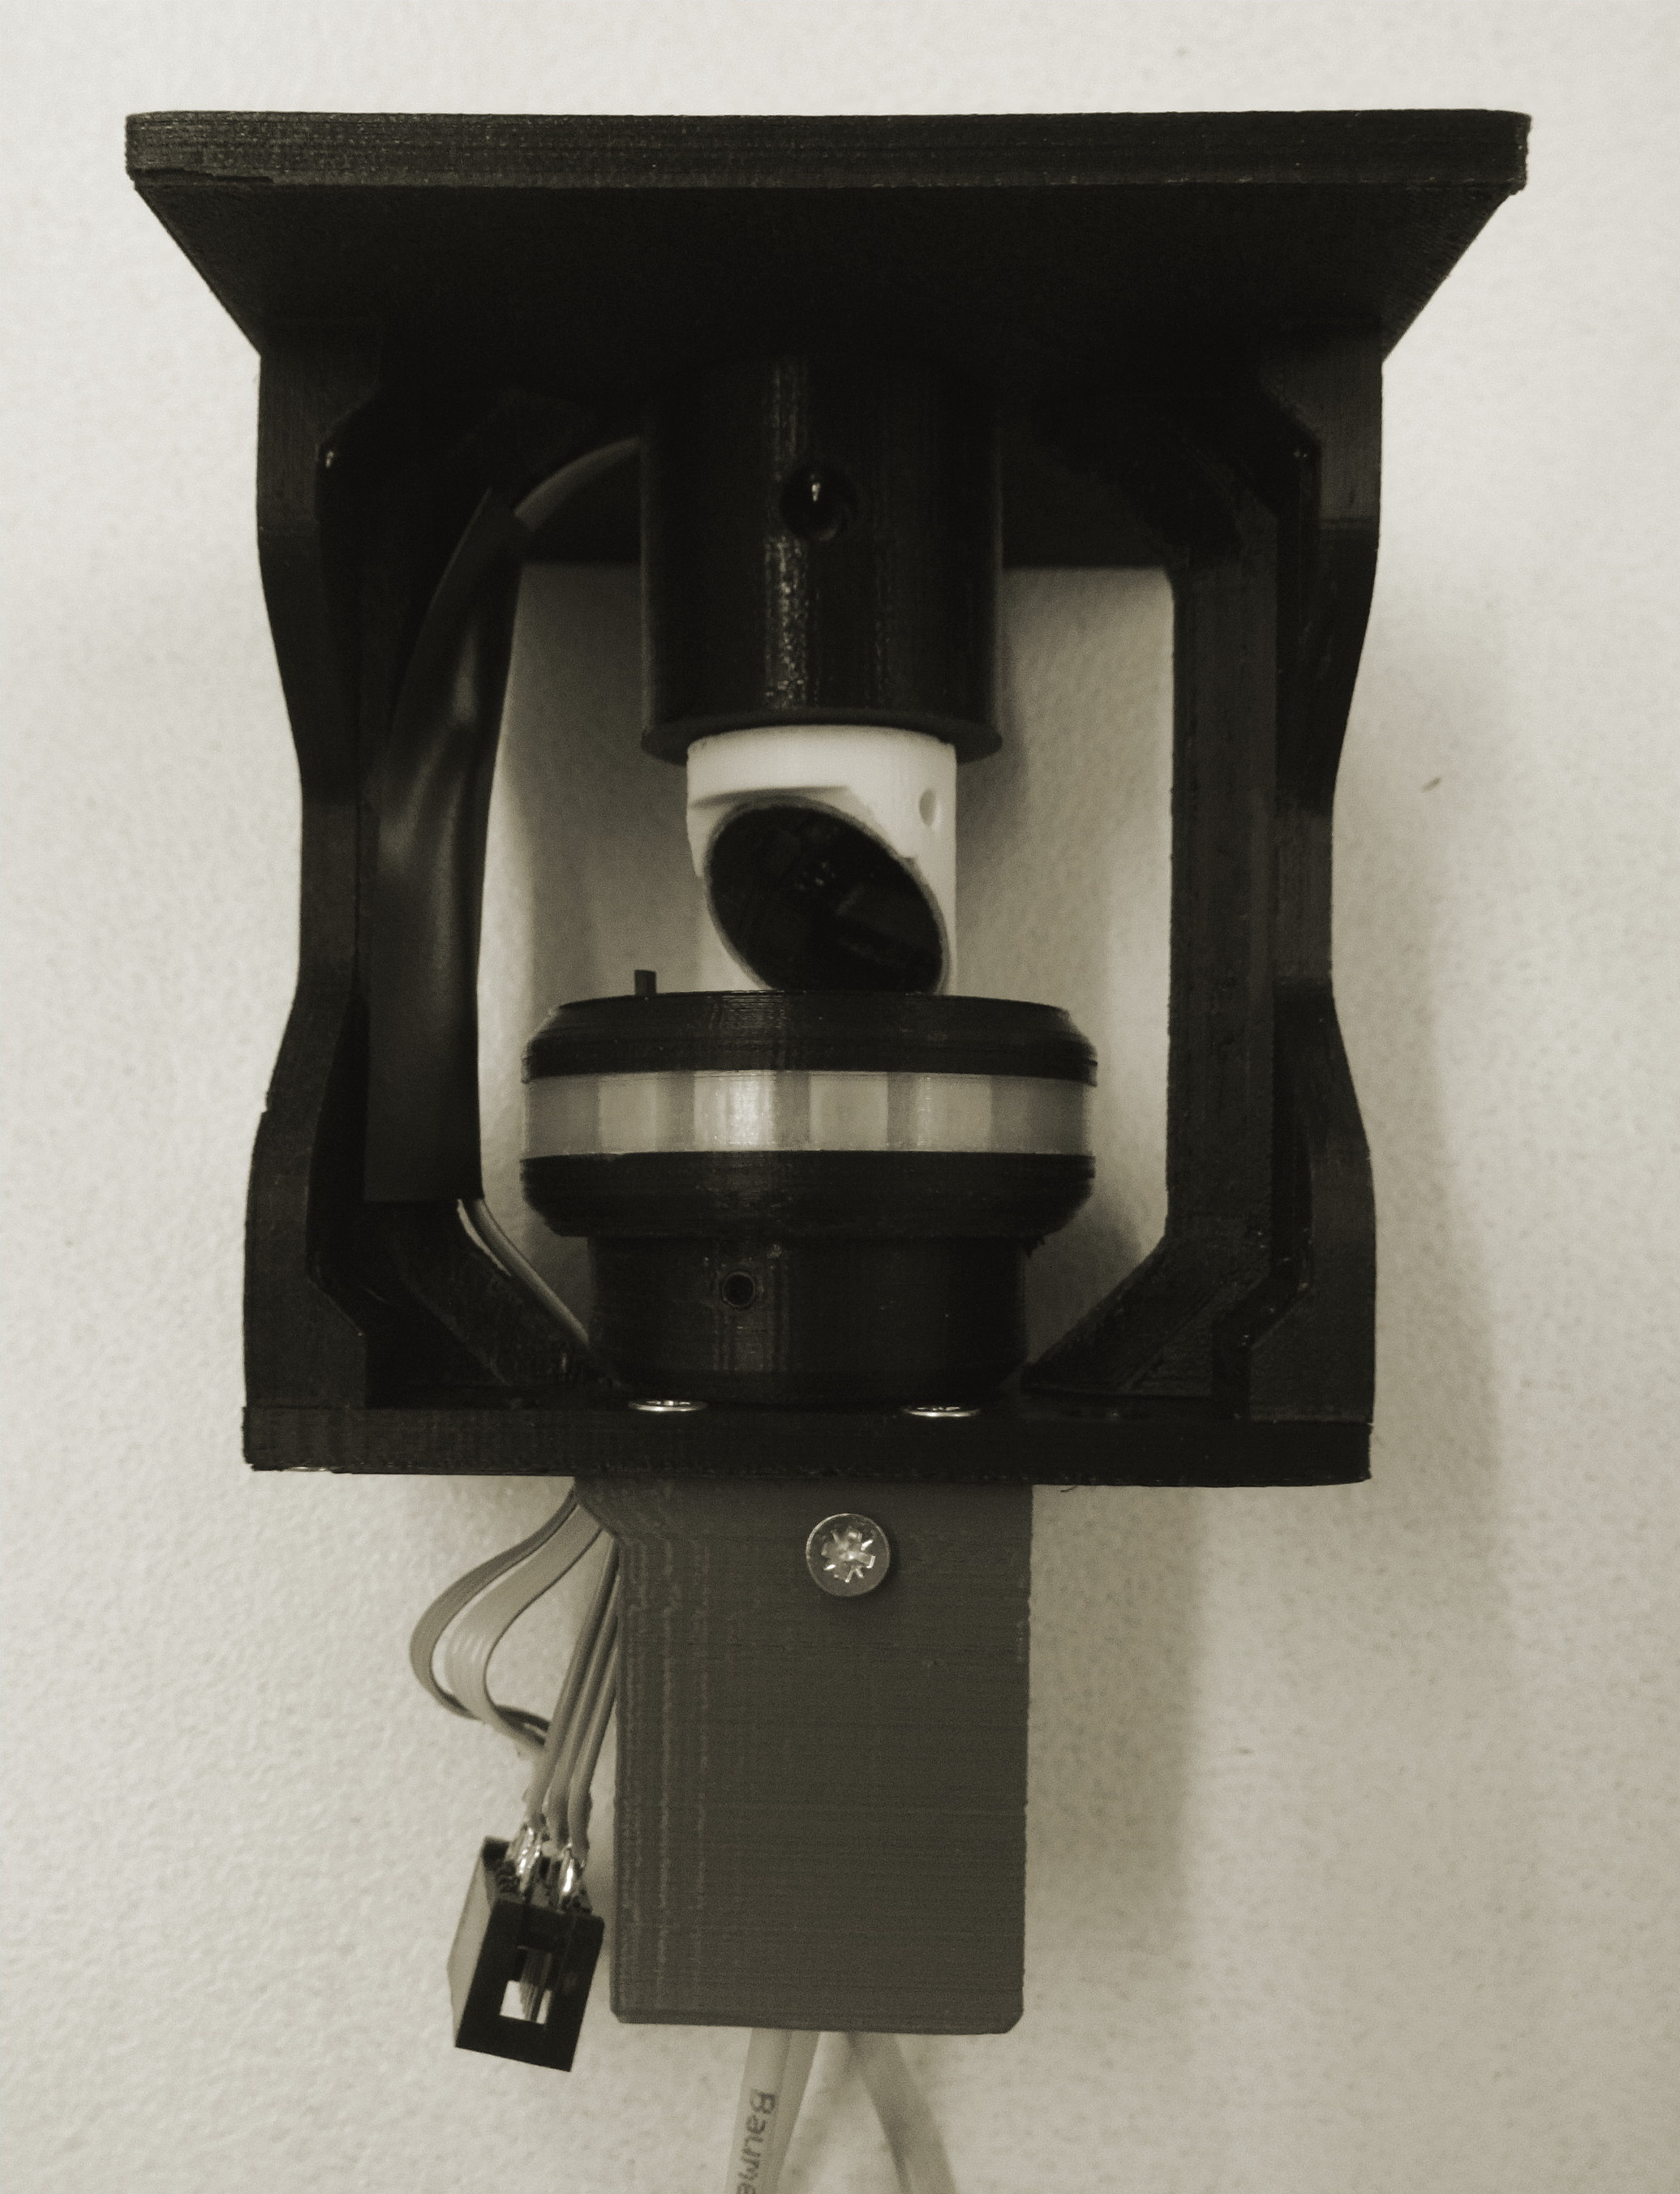
\includegraphics[height=\height] {../images/OD/Kopf3Pres.JPG}};
		\begin{scope}[x={(rimage.south east)},y={(rimage.north west)} ]
		
			\draw [line width=0.4mm, ->, cGreen] (0.5,1.02) node[above, color=black]{Motor und Spiegel} -- (0.5, 0.8);
			\draw [line width=0.4mm, ->, cGreen] (0.55,-0.1) node[right, color=black]{LED-Ring} -- (0.55, 0.4);
			
			\draw [line width = 0.6mm, -, cRed] (-0.32, -0.1985) to[out = 0, in = 270] (0.32, 0.1);
			\draw [line width = 0.4mm, -, cRed] (-0.49, 0.87) -- (-0.49, 0.44);
			\draw [line width = 0.6mm, -, cRed] (-0.49, 0.655) to[out = 0, in = 90] (-0.2, 0.44);
			\draw [line width = 0.6mm, -, cRed] (-0.2, 0.44) -- (-0.2, 0.0);
			\draw [line width = 0.6mm, -, cRed] (-0.2, 0.0) to[out = 270, in = 270] (0.5, 0.0);
		
		\end{scope}
	\end{scope}
	\end{tikzpicture}	
\end{figure}

\end{frame}

\begin{frame}
	\frametitle{Gegnererkennung}
	\framesubtitle{Ausmessung Spiegelhalter}
	
	\begin{figure}
		\centering
		\begin{tikzpicture}[y=-1cm, scale=0.5, transform shape]
		%near right
		\draw [draw=cRed, fill=clRed, fill opacity=0.3] (300:0.6) -- (300:1.95) -- (330:1.65) -- (0:1.6) -- (30:1.8) -- (60:2.4) -- (60:0.8) -- (30:0.65) -- (0:0.5) -- (330:0.5) -- (300:0.6);		
		%middle right
		\draw [draw=cBlue, fill=clBlue, fill opacity=0.3] (300:0.95) -- (330:0.93) -- (0:0.88) -- (30:0.85) -- (60:0.8) -- (60:2.75) -- (30:3.1) -- (0:3.05) -- (330:3.1) -- (300:3.05) -- (300:0.95);
		%middle left
		\draw [draw=cBlue, fill=clBlue, fill opacity=0.3] (120:0.73) -- (150:0.73) -- (180:0.75) -- (210:0.78) -- (240:0.88) -- (240:2.65) -- (210:2.8) -- (180:2.65) -- (150:2.35) -- (120:2.35) -- (120:0.73);
		%far right
		\draw [draw=cGreen, fill=clGreen, fill opacity=0.3] (300:1.25) -- (330:1.25) -- (0:1.1) -- (30:1) -- (60:0.88) -- (60:3.15) -- (30:4.2) -- (0:4.95) -- (330:4.9) -- (300:5) -- (300:1.5);
		
		%far left
		\draw [draw=cGreen, fill=clGreen, fill opacity=0.3] (120:0.65) -- (150:0.55) -- (180:0.6) -- (210:0.7) -- (240:0.83) -- (240:2.9) -- (210:2.25) -- (180:2) -- (150:1.75) -- (120:1.85) -- (120:0.65);
		%middle left
		\draw [draw=cBlue, fill=clBlue, fill opacity=0.3] (120:0.73) -- (150:0.73) -- (180:0.75) -- (210:0.78) -- (240:0.88) -- (240:2.65) -- (210:2.8) -- (180:2.65) -- (150:2.35) -- (120:2.35) -- (120:0.73);
		% near left
		\draw [draw=cRed, fill=clRed, fill opacity=0.3] (120:1.4) -- (150:1.7) -- (180:1.75) -- (210:1.65) -- (240:1.25) -- (240:4.25) -- (210:5) -- (180:5) -- (150:5) -- (120:5) -- (120:1.4);
		
		%draw Coordinate System
		\foreach \phi/\t in {0/90,30/120,60/150,90/180,120/210,150/240,180/270,210/300,240/330,270/0,300/30,330/60}
		{
			\draw [color=cGray] (0,0) -- (\phi:5.5);
			\node [fill=white] at (\phi:5.7) {\t°};
		}
		\foreach \r in {1,1.5,2,2.5,3,3.5,4,4.5,5}
		{
			\draw [color=cGray] (0,0) circle (\r);
		}
		\foreach \t/\x in {200/1,400/2,600/3,800/4,1000/5}
		{
			\node [fill=white, rounded corners=2mm] at (270:\x) {\t};
		}
		
		\draw [thick, ->] (0:7) -- (0:9) node[pos=0.5, above] {Vorwärts};
		
		\end{tikzpicture}
	\end{figure}

\end{frame}
  
  %Fahrkontroller
  \section{Fahrcontroller}

\begin{frame}
	\frametitle{Anpassungen}	
	\begin{columns}
		\begin{column}{0.6 \textwidth}
			\begin{itemize}
				\item Studienarbeit als Basis
				\item Interface auf Mainboard
				\item Kommunikation
				\item Rest bei Gleitkommaoperationen
				\item Kalibrierung
			\end{itemize}
		\end{column}
		\begin{column}{0.4 \textwidth}
			\vspace{-2.8em}
			\begin{figure}[h]
				\centering
				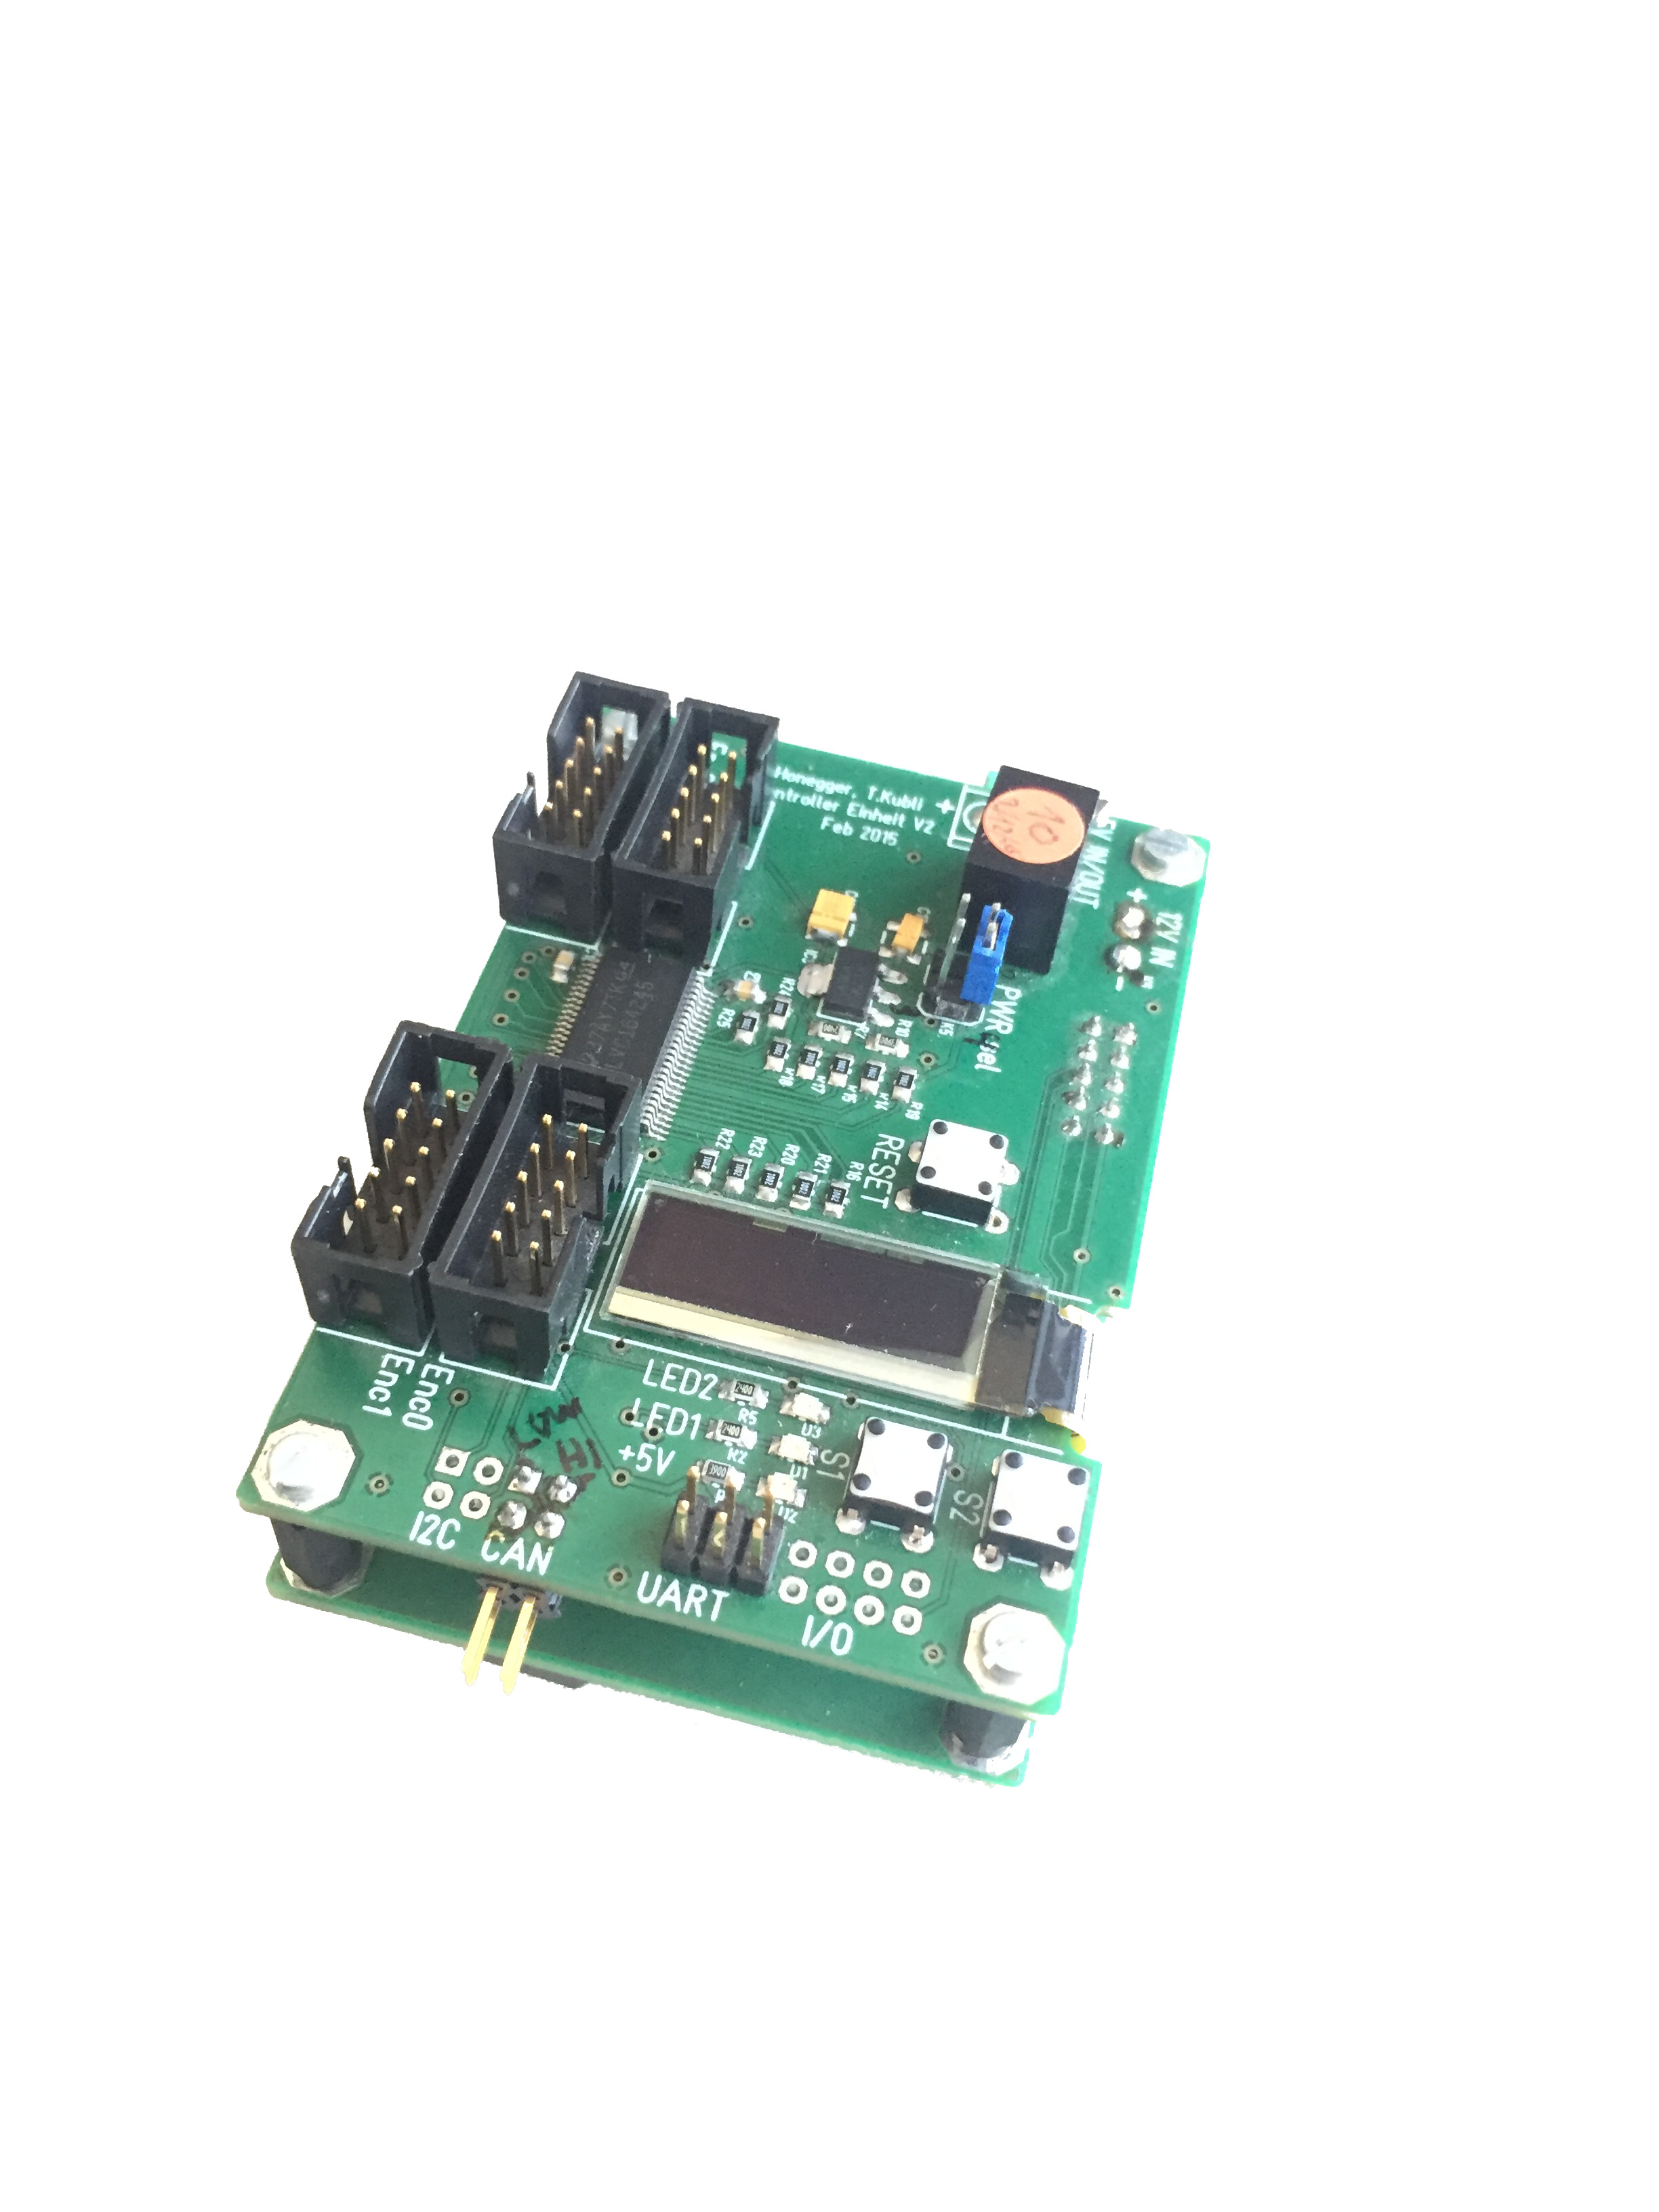
\includegraphics[width = 1 \textwidth]{../images/presentation/dc.jpg}
			\end{figure}
		\end{column}
	\end{columns}
	

\end{frame}

\begin{frame}
	\frametitle{Kalibrieren}
	\begin{itemize}
		\item verbesserte Fehlerberechnung
		\item Bedienung über Display
		\item Konfigurationsdaten auf USB-Stick
		\item getrennte Kalibrierung für Vorwärts- und Rückwärtsfahrt
	\end{itemize}
\end{frame}

\begin{frame}
	\frametitle{Probleme}
	\begin{itemize}
		\item Synchronisation schwierig
		\item kein vorausschauendes Fahren
		\item ungenaues Fahren
		\item Reglereinstellung mühsam
	\end{itemize}
\end{frame}
 
  %Fazit
  \section{Fazit}
\begin{frame}
\frametitle{Fazit}

\begin{itemize}
	\item Viele Ziele erreicht
	\item Einiges gelernt
	\item Sinnvolle Aufgabenteilung
	\item Harmonierendes Team
\end{itemize}
\end{frame}    
  
\end{document}
